\documentclass[Thesis]{subfiles}

\begin{document}

\newpage
\chapter{Smoothing, decomposing and forecasting mortality rates}\label{Ch6}
\thispagestyle{empty}
\pagecolor{pagecolor}\afterpage{\nopagecolor}
\vspace{1cm}
\Large
Carlo Giovanni Camarda\\
Ugofilippo Basellini
\vspace{2cm}
\\ Manuscript under review.\\

\clearpage

\thispagestyle{empty}
\pagecolor{pagecolor}\afterpage{\nopagecolor}
\section*{}
\clearpage

% % --------------------------------------------

\thispagestyle{empty}
{\centering
{\Large\bfseries Smoothing, decomposing and forecasting mortality rates \par}
\vspace{0.5cm}
{\large Carlo Giovanni Camarda$^{1,\dagger}$ and Ugofilippo Basellini$^{1,2}$ \par}
\singlespacing
{\normalsize $^{1}$\itshape Institut national d'\'{e}tudes d\'emographiques (INED), Paris, France\\[2mm]}
{\normalsize $^{2}$\itshape Interdisciplinary Centre on Population Dynamics (CPop) and Department of Public Health, University of Southern Denmark, Odense, Denmark\\[2mm]}
{\normalsize $^{\dagger}${\itshape Corresponding author:} \url{carlo-giovanni.camarda@ined.fr} \par}
\vspace{2.0cm}
{\bfseries Abstract \\[5mm]}
{\normalsize \justify The Lee-Carter (LC) model represents a landmark paper in mortality forecasting. Whilst having been widely accepted and adopted, the model has some limitations that hinder its performance. Some variants of the model have been proposed to deal with these drawbacks individually, none coped with them all at the same time. In this paper, we propose a Three-Component smooth Lee-Carter (3C-sLC) model which overcomes all the issues simultaneously. It decomposes mortality development into childhood, early-adult and senescent mortality, which are described, individually, by a smooth variant of the LC model. Smoothness is enforced to avoid irregular patterns in projected life tables, and complexity in the forecasting methodology is unaltered with respect to the original LC model. Component-specific schedules are considered in projections, providing additional insights into mortality forecasts. We illustrate the proposed approach to mortality data for the USA and Switzerland. The 3C-sLC captures mortality developments better than a smooth improved version of the LC model, and it displays wider prediction intervals. The proposed approach provides demographers, actuaries, epidemiologists and social scientists in general with a unique and valuable tool to simultaneously smooth, decompose and forecast mortality.   \par 
\vspace{0.5cm}	
\noindent \textbf{Keywords:} mortality decomposition$\;\cdot\;$mortality forecasting$\;\cdot\;$smoothness$\;\cdot\;$rate of mortality improvement$\;\cdot\;$Lee-Carter model}	
}

\newpage

% --------------------------------------------

\normalsize

\section{Background}\label{Sec:Ch6sec1}
An accurate knowledge of future mortality patterns and their uncertainty is crucial in almost all areas of a society, including the health-care system, health and life insurance, as well as pension schemes. Since \cite{bonynge1852future}, demographers, actuaries and statisticians have developed several methodologies and techniques to predict mortality. However, up until the 1980s, mortality forecasts were based on deterministic scenarios and, generally, some variants would be assumed at the life expectancy level as input for producing population projections. This approach was used almost without exception by international bodies, such as the United Nations and World Bank, and national statistical offices \citep{booth2006demographic}. 

One of the main limitations of this scenario-based approach is that the probability of different scenarios cannot be quantified nor specified a priori, and the structure of mortality developments over age and time is only partially considered. For this reason, the last thirty years witnessed an increasing use of more sophisticated statistical methodologies for projections, which enable the construction of forecast probability distributions and probabilistic prediction intervals, mainly using time changes in age-specific death rates \citep{booth2008mortality}.

The use of stochastic models has flourished in recent decades \citep[for comprehensive reviews, see][]{booth2006demographic,booth2008mortality, stoeldraijer2013impact} and in \citeyear{lee1992modeling}, a breakthrough was achieved by \citeauthor{lee1992modeling}, who proposed an elegant and powerful methodology to forecast mortality that later became widely accepted and employed. The Lee-Carter (LC) model is based on linear extrapolations of the logarithms of age-specific death rates, using principal component techniques. In particular, a matrix of logged age-specific mortality rates over time is summarized by two vectors of age-specific parameters $\alpha_x$ and $\beta_x$, which describe the general shape of mortality and the fixed rate of mortality improvement at age $x$, respectively, and by a time-varying index $\kappa_t$, which captures the general level of mortality. Mortality forecasts are then derived from the projection of $\kappa_t$ using standard time series methods.

While the LC model works reasonably well, several limitations have been revealed in the succeeding literature. A central assumption of the LC model is the fixed rate of age-specific mortality improvement over time \citep{lee2001evaluating}. Already recognized by \citet{alho1992comment}, this assumption has been violated in several low-mortality countries in recent decades, as rates of mortality improvements have tended to decline over time at younger ages, and they have risen at older ages \citep{kannisto1994reductions, vaupel1998biodemographic, wilmoth1999rectangularization}. As a result, projections that ignore this ``rotation'' of mortality declines will lead to errors, particularly in the projected age patterns of future death rates. To overcome this limitation, \cite{li2013extending} proposed a rotation of the $\beta_x$ schedule for long-term projections. This allows one to capture the observed trend of deceleration of infant and child mortality decline and the acceleration of old-age mortality reduction in low-mortality countries during the most recent decades. A similar approach has been used in other projection models \citep{sevcikova2016agespecific}. Nevertheless, the approach proposed by \cite{li2013extending} relies strongly on a subjective choice of the model parameters, and it does not account for the stochastic process behind mortality.

The original LC model is estimated by minimizing the residual sum of squares using singular value decomposition (SVD), which is as simple as inappropriate when dealing with mortality data \citep{wilmoth1993computational, dejong2006extending, koissi2006fuzzy}. \cite{brouhns2002poisson} embedded the LC model within a Poisson setting using Maximum Likelihood Estimation and a Newton-Raphson algorithm to estimate model parameters. Other papers used this Poisson assumption for estimating the LC model \citep{renshaw2003leecarterAPPSTAT, brouhns2005bootstrapping, czado2005bayesian, haberman2008mortality, li2017optimizing}. Despite the appropriate estimation procedure, the LC model leads to outcomes which become less smooth and more unrealistic when projected, and age-patterns tend to deviate from any given baseline described by $\alpha_{x}$ \citep{girosi2007understanding, girosi2008demographic}. To prevent irregular projected life tables, smoothing techniques have been implemented within an LC framework. Whereas \cite{renshaw2003forecasting} suggested smoothing estimated series of $\beta_{x}$, \cite{hyndman2007robust} employed a functional data approach and smoothed the mortality data as a preliminary step. Alternatively, a penalized likelihood approach has been proposed by \cite{delwarde2007smoothing} and \cite{currie2013smoothing}. Their approach allows them to frame the LC model within a Poisson setting and simultaneously obtain smooth $\beta_{x}$ and, consequently, regular forecast age-patterns. 

None of the variants and generalizations of the LC model attempted to account for the complex nature of the human mortality age-pattern. Specifically, we refer to the hypothesis that human mortality can be decomposed into three different groups that operate principally upon childhood, middle and old ages, respectively. This idea goes back at least one and a half centuries \citep{thiele1871mathematical} and it leads to a so-called "bath-tub shaped" mortality age-pattern. In most developed populations, during the first years of life, mortality decreases steeply from a relatively high value at age 0 \citep{levitis2011before}. A minimum is commonly reached at ages around 10-15 \citep{ebeling2018how}. Afterwards, especially for men, hazard rates show a hump at young-adult ages \citep{goldstein2011secular, remund2015jeunesses}. Starting from about age 30, mortality rises exponentially and eventually it tends to level off at ages above 80 \citep{PrestonMortPattern1976, vaupel1997trajectories, thatcher1998force}. The idea of mortality constructed from three competing components has been extensively used for modeling purposes \citep{siler1979competing,siler1983parameters,heligman1980age, kostaki1992nine, rogers1994parameterizing,dellaportas2001bayesian, de2016new, camarda2016sums, mazzuco2018mortality, remund2018young}. However, very few attempts have been made to forecast the three components. Only \cite{forfar1987changing} employed the \citeauthor{heligman1980age} model for forecasting, as the large number of parameters limits the model's potential for projections \citep{mcnown1992forecasting}. In addition, the model's parameters are typically highly correlated \citep{hartmann1987past}, and these high correlations further compromise their interpretability \citep{booth2008mortality}.

Here, we propose a novel extension of the LC model that (i) is framed within a Poisson setting; (ii) enforces smoothness in the outcomes and (iii) addresses the drawback of the fixed rates of mortality improvement from a different perspective, i.e.~by separately modeling childhood, early-adult and high-ages mortality. In particular, we simultaneously estimate a smooth variant of the LC model for all three components of human mortality. We therefore call our approach the "Three-Component smooth Lee-Carter" (3C-sLC) model. In other words, given a set of observed death counts and exposure-to-risk data, we derive the standard LC parameters $\alpha_x$, $\beta_x$ and $\kappa_t$ for each component, with both $\alpha_x$ and $\beta_x$ smoothly varying over $x$. Forecasting is achieved by extrapolating component-specific time-indexes via standard Box-Jenkins methods, maintaining the simplicity of the original LC model in projecting future trends.  The main advantage of our model is the greater flexibility of mortality patterns, which do not depend on a single fixed rate of age-specific mortality improvement, but rather on the combination of different component-specific schedules.  The methodology that we propose also allows us to forecast overall mortality as a sum of future component-specific patterns. Consequently, future trends in childhood, early-adult and old-age mortality can be analyzed independently, adding great explanatory value to the proposed approach. 

This paper is organized as follows. In Section \ref{Sec:Ch6sec2}, we start by introducing the data that we use in the paper, which are derived from the \cite{HMD}. We present the original LC model and its smooth version in Section \ref{Subsec:Ch6subsec2.1}; then, Section \ref{Subsec:Ch6subsec2.2} introduces the 3C-sLC model, as well as the procedures for estimating its parameters and obtain mortality forecasts. Throughout Section \ref{Sec:Ch6sec2}, we present outcomes of the smooth LC and 3C-sLC models on a specific population for illustrative purposes. In Section \ref{Sec:Ch6sec3}, we show and compare the results of fitting and forecasting mortality in four populations using the two models. Section \ref{Sec:Ch6sec4} provides a discussion of our methodology and its related results, and Section \ref{Sec:Ch6sec5} concludes the paper. 


\section{Data and methods}\label{Sec:Ch6sec2}

We assume that we have data on deaths and exposures to the risk of death, arranged in two matrices, $\bm{Y} = (y_{x,t})$ and $\bm{E} = (e_{x,t})$, each $m \times n$ where rows and columns are classified by single age at death, $\bm{x}, \,m \times 1$, and single year of death, $\bm{t}, \,n \times 1$, respectively. We aim to forecast mortality for future years $\bm{t}_{F}, \,n_{F} \times 1$.
We assume that the number of deaths $y_{x,t}$ are realizations of the random variable $Y_{x,t}$, which follows a Poisson distribution:
\begin{equation}\label{eq:Poisson}
Y_{x,t} \sim \mathcal{P}(e_{x,t}\,\mu_{x,t}) \, ,
\end{equation}
i.e.~the expected value is the product of exposures and the force of mortality \citep{brillinger1986biometrics}. Description of the mortality development over age and time is commonly provided by portraying the so-called death rates: $m_{x,t}= y_{x,t}/e_{x,t}$. 

\begin{figure}[!ht]\centering
	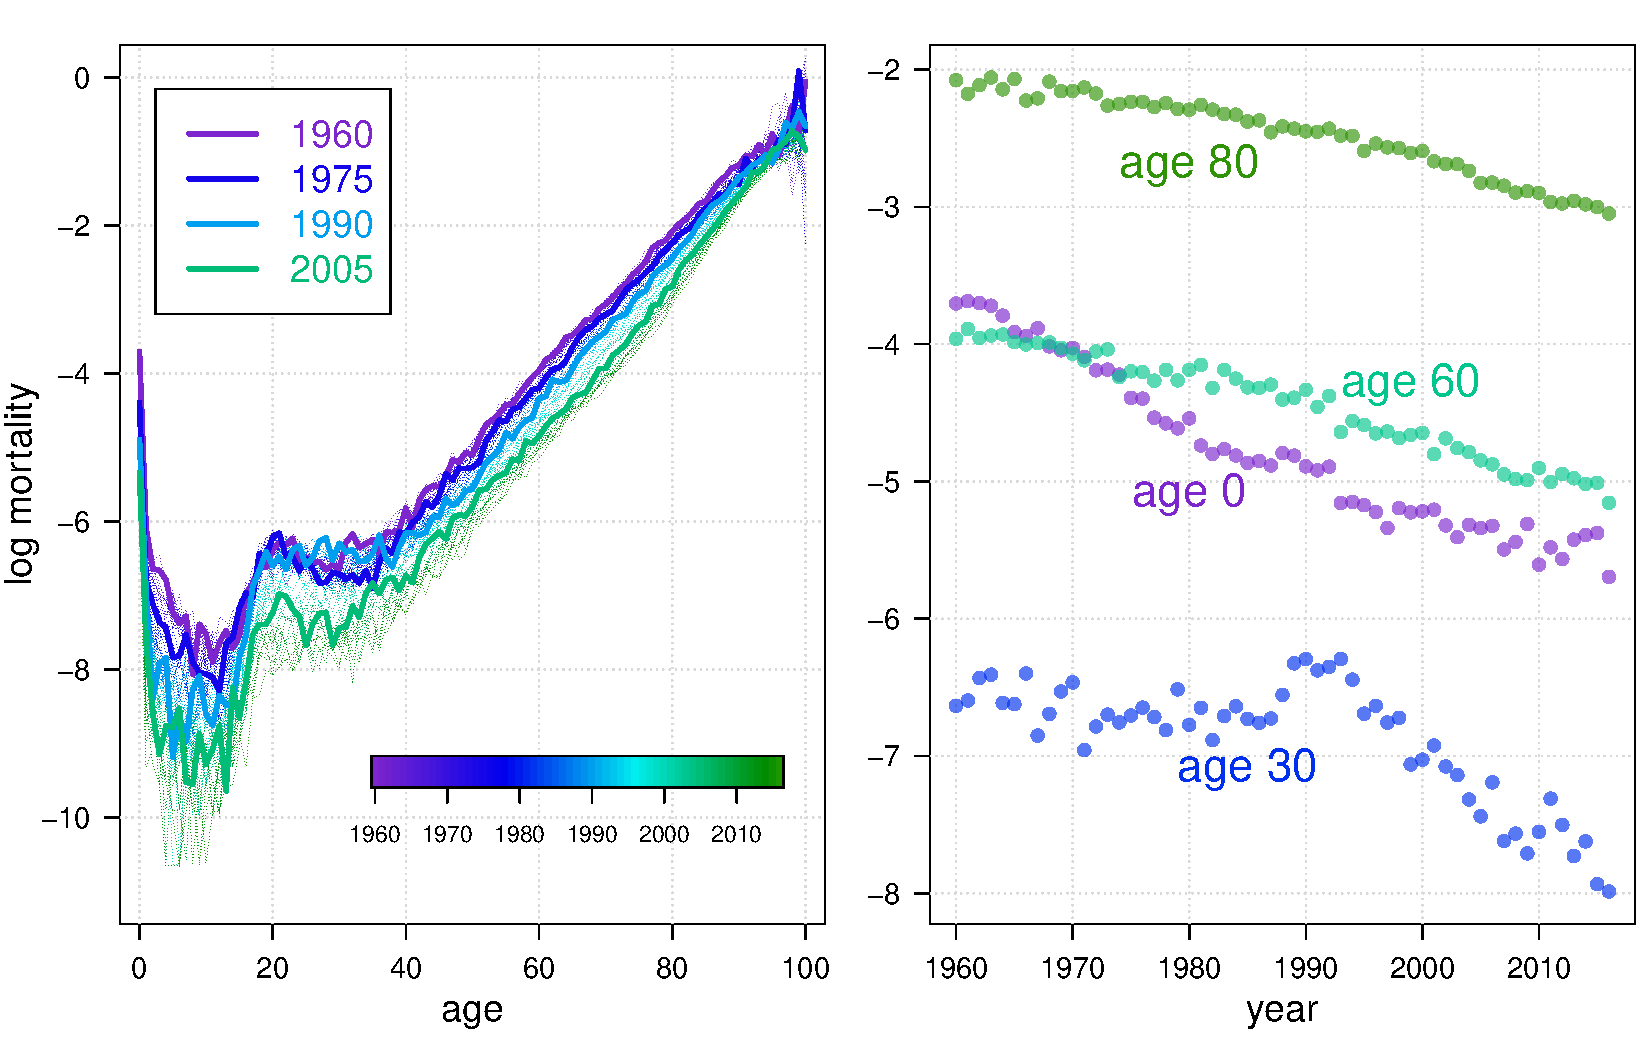
\includegraphics[scale=0.52]{./Ch6/DataCHE.pdf}
	\caption{\label{fig:DataCHE} Actual death rates over age and time on a log scale for Swiss males. Ages 0-100, years 1960-2016. Left panel: rates over age for all years. Selected years are depicted by thicker lines. Right panel: selected ages over years.}  
\end{figure}

In the following, we will present outcomes from the proposed model for four different populations. Specifically, we analyze both female and male populations of the USA and Switzerland (CHE). Data are taken from the \citet{HMD}. We model mortality from ages 0 to 100 over the period 1960-2016, forecasting up to 2050.

In this section and only for illustrative purposes, methodology is presented on Swiss males data. Figure~\ref{fig:DataCHE} shows mortality rates on a log scale over ages for all years as well as time trends for selected ages over time. The typical mortality age-pattern is portrayed in the left panel: a rapid declining mortality from birth, a roughly log-linear trajectory starting from ages 30-40, and an intermediate phase in early-adult ages often described as "accident hump". 

Time trends are also identifiable in the right panel of Figure~\ref{fig:DataCHE}. A general mortality improvement is clear with decreasing rates over time. However, differences in the speed of mortality reductions are evident for different ages, and some ages have also experienced stagnation and increasing mortality, e.g.~age 30 from 1960 to early 1990s. Whereas looking at death rates helps to have a good image of mortality developments, it is essential to develop statistical models to obtain an accurate and parsimonious description as well as a reliable prediction of the observed trends. The following pages will be devoted to this purpose. 

\subsection{The Lee-Carter model}\label{Subsec:Ch6subsec2.1}

\cite{lee1992modeling} pioneered an elegant and powerful methodology to model and forecast mortality based on a simple formula for the logged death rates:
\begin{equation}\label{eq:Lee-Carter}
\ln (m_{x,t}) =\alpha_x+\beta_x \, \kappa_t + \varepsilon_{x,t} \, ,
\end{equation}
where $\alpha_x$ describes the average shape of the age profile, $\beta_x$ the rate of mortality improvement at age $x$, and $\kappa_t$ the general level of mortality at time $t$. The $\varepsilon_{x,t}$ are error terms that reflect residual age-specific historical influences not captured by the model. To ensure model identification, the parameters are commonly subjected to the following constraints:
\begin{equation}\label{eq:Lee-Carter_constr}
\sum_{x} \beta_x = 1 \quad \mathrm{and} \quad \sum_{t} \kappa_t = 0\, .
\end{equation}

The original Lee-Carter (LC) model is estimated by minimizing the residual sum of squares:
\begin{equation}\label{eq:Lee-Carter_RSS}
\sum_{x,t} \left( \ln (m_{x,t}) -\alpha_x - \beta_x \, \kappa_t \right)^2 \, .
\end{equation}
In particular, the authors employ a singular value decomposition (SVD) method to find the least squares solution of \eqref{eq:Lee-Carter_RSS}; as such, the estimated $\hat{\alpha}_x$ is the average of the observed $\ln (m_{x,t})$, while $\hat{\beta}_x$ and $\hat{\kappa}_t$ are the first left- and right-singular vectors of the SVD of the matrix $\ln (m_{x,t}) - \hat{\alpha}_x \,$. Furthermore, the parameter $\hat{\kappa}_t$ is adjusted in a second-step estimation so that the resulting fitted deaths match the total number of deaths observed in the data at each year $t$.

An advantage of the LC model is that its time-index $\kappa_{t}$ can be easily forecast since it is able to capture the linear decline of the observed mortality development: see the grey dashed line in the right panel of Figure \ref{fig:LC3CPAR} (note that the figure also plots parameters of our proposed model, which should be ignored for now). In particular, forecasting in the LC model is performed by modelling and extrapolating fitted values of $\kappa_{t}$ by an autoregressive integrated moving average (ARIMA) process. A random walk with drift (RWD) is used almost exclusively in applications with low-mortality populations and in the following we will follow this approach. Finally the extrapolated $\kappa_{t}$ and its uncertainty are combined with the previous estimations to forecast the future death rates and associated prediction intervals.

With respect to the estimation procedure, the main drawback of the ordinary least-squares estimation via SVD is that the errors are assumed to be homoskedastic and normally distributed, which is a fairly unrealistic assumption for human mortality \citep{alho2000discussion}. Indeed, the logarithm of the observed force of mortality is much more variable at older than at younger ages because of the much smaller number of deaths \citep{brouhns2002poisson}. 

To overcome this limitation, \cite{brouhns2002poisson} embed the LC model in a Poisson setting. The logarithm of the force of mortality in \eqref{eq:Poisson} can then be written as follows:
\begin{equation}\label{eq:LCmu}
\ln(\mu_{x,t}) = \alpha_{x} + \beta_{x}\kappa_{t}
\end{equation}
or in matrix notation:
\begin{equation}\label{eq:LCmatrix}
\ln \bm{M} = \bm{\alpha}\,\bm{1}'_{n} + \bm{\beta}\,\bm{\kappa}'\,  
\end{equation}
where $\bm{M} = (\mu_{ij})$ is the matrix of the underlying force of mortality, $\bm{\alpha}$, $\bm{\beta}$ and $\bm{\kappa}$ denote the LC parameter-vectors and $\bm{1}_{n}$ is a $n \times 1$ matrix of 1s. 
Estimates of the parameters can be achieved by maximizing the associated log-likelihood function:
\begin{equation}\label{eq:PoiLogLike}
\ln\mathcal{L}\left(\bm{\alpha}, \bm{\beta}, \bm{\kappa} | \, \bm{Y} , \bm{E}\right) \propto \sum_{x,t} \left[ y_{x,t} \, \ln \left ( \mu_{x,t}  \right ) - e_{x,t}
\, \mu_{x,t} \right]  \, . 
\end{equation}
The model parameters are subject to the same constraints as in~\eqref{eq:Lee-Carter_constr} and the log-likelihood in \eqref{eq:PoiLogLike} is maximized by a uni-dimensional iterative Newton-Raphson method. The advantage of this assumption is that the error terms in the model now follow a non-additive heteroscedastic error structure, which is more appropriate for modeling human mortality. Moreover maximum-likelihood estimation does not require any second-step adjustment of $\hat{\bm{\kappa}}$, as the fitted number of deaths already matches the observed deaths at each year $t$.

Regardless of the estimation procedure, irregular age-patterns in future mortality have been observed when the LC model has been used, and increasing loss of smoothness over ages is a well known feature of this model \citep{girosi2007understanding, girosi2008demographic}. This is mainly due to the $\bm{\beta}$, which often exhibits a fluctuating pattern that results in irregular projected life tables. Instead of smoothing the estimated $\bm{\beta}$ without modifying $\bm{\alpha}$ and $\bm{\kappa}$, \citet{delwarde2007smoothing} proposed a penalized likelihood approach to obtain smooth $\bm{\beta}$ within the estimation procedure. In addition, we propose smoothing the parameter-vector $\bm{\alpha}$ since, especially in small populations, the simple average mortality age-pattern might present variable behaviour that can contribute to produce unsmooth future mortality patterns. In contrast, the time-index $\bm{\kappa}$ is free to vary over the years to better capture mortality fluctuations and provide an appropriate measurement of the uncertainty when forecasting is involved. 

Smooth LC estimates could be achieved by adding a penalty term in the log-likelihood~\eqref{eq:PoiLogLike} which penalizes differences between adjacent $\bm{\alpha}$ and $\bm{\beta}$:
\begin{equation}\label{eq:PoiPenLogLike}
\ln\mathcal{L}^{P}\left(\bm{\alpha}, \bm{\beta}, \bm{\kappa} | \, \bm{Y} , \bm{E}\right) = \ln\mathcal{L}\left(\bm{\alpha}, \bm{\beta}, \bm{\kappa} | \, \bm{Y} , \bm{E}\right) - \frac{1}{2} \,\lambda_{\alpha} \, \bm{\alpha}' \,\bm{D}'\bm{D} \, \bm{\alpha} - \frac{1}{2} \,\lambda_{\beta} \, \bm{\beta}' \,\bm{D}'\bm{D} \, \bm{\beta} 
\end{equation}
where the smoothing parameters $\lambda_{\alpha}$ and $\lambda_{\beta}$ control the amount of smoothness in the vector $\bm{\alpha}$ and $\bm{\beta}$ and $\bm{D}$ is the second order difference $m \times (m-2)$ matrix:
\begin{equation}\label{eq:D}
\bm{D} = \begin{brmatrix}[1em]
1 & -2 & 1 & 0 & 0 & \cdots \\
0 & 1 & -2 & 1 & 0 & \cdots \\
0 & 0 & 1 & -2 & 1 & \cdots \\
\vdots & \vdots & \vdots & \vdots & \vdots & \ddots\\
\end{brmatrix}\, .
\end{equation}
The order of difference in $\bm{D}$ does not play a relevant role in this context. Unless specified otherwise, in the following we use second order differences. Moreover we can use the same $\bm{D}$ matrix for both parameter-vectors since they both act on the age dimension. 

In other words, the larger the smoothing parameters $\lambda_{\alpha}$ and $\lambda_{\beta}$, the smoother the estimates of $\bm{\alpha}$ and $\bm{\beta}$, respectively. Consequently fitted rates will show smoother patterns. Alternatively small $\lambda$s lead to estimates close to the original LC model. Here we optimized both smoothing parameters by minimizing the Bayesian Information Criterion \citep[BIC,][]{schwarz1978estimating}. 

Gray dashed lines in Figure~\ref{fig:LC3CPAR} present estimated parameters from this smooth variant of the Lee-Carter model for Swiss males. The vector $\bm{\alpha}$ shows the average mortality age-pattern, and the accident-hump is evident for early adult ages. This average trajectory is modulated over age and time by the parameters $\bm{\beta}$ and $\bm{\kappa}$, respectively. A general linear time-trend is visible in the right panel and the average mortality improvement described by $\beta_{x}$ presents large changes in younger ages and about age 70. 

The time index is then extrapolated using a RWD and associated prediction intervals can be computed (grey areas in the right panel of Figure \ref{fig:LC3CPAR}). From estimated and future values of $\kappa_{t}$ as well as estimated $\bm{\alpha}$ and $\bm{\beta}$, the whole mortality development over both age and time is computed. 

Figure~\ref{fig:LCsmoOUT} shows estimated and forecast death rates on a log scale for Swiss males. Whereas the smooth Lee-Carter is able to capture the general mortality improvement, future age-patterns still show fluctuating behaviour. Moreover, the fixed age-specific average rates of mortality improvement, described by the vector $\bm{\beta}$, lead to unreasonable time-trends, i.e.~all age groups show a constant decline in mortality that has not been observed in the past decades. These features are ultimately translated into future age-patterns that produce a poor description of past trends; see especially the fitted mortality for ages 0 and 30.

\begin{figure}[!ht]\centering
	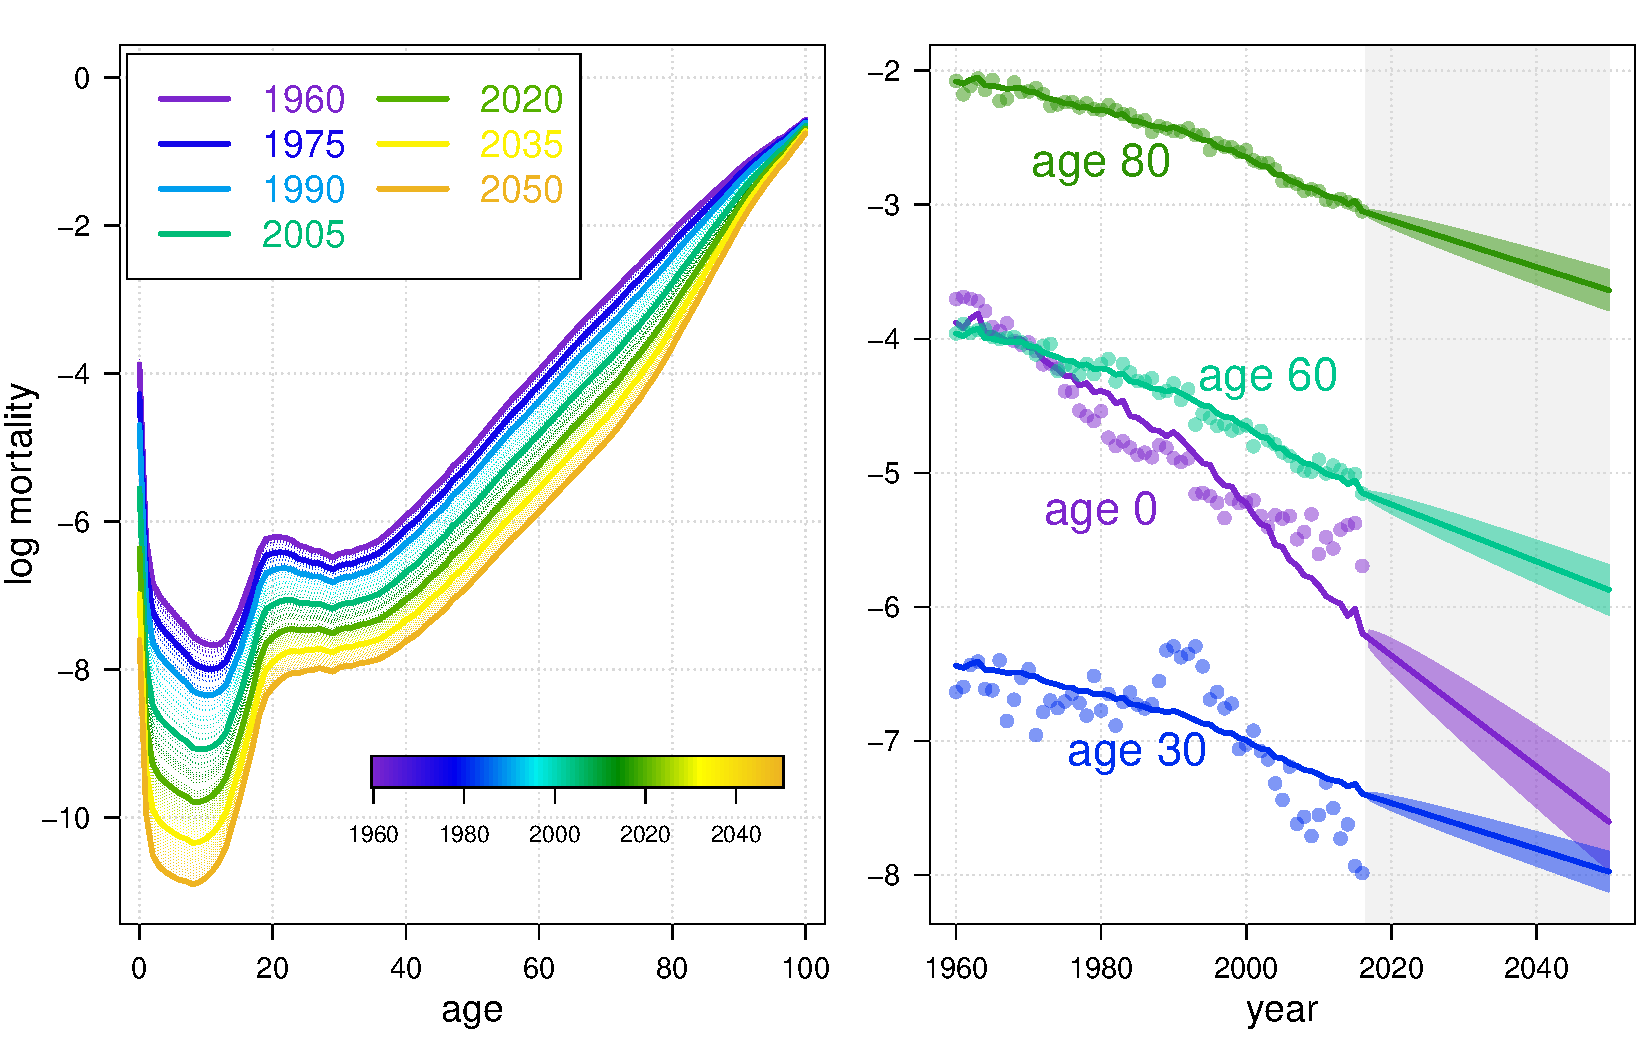
\includegraphics[scale=0.52]{./Ch6/LCsmoOUT.pdf}
	\caption{\label{fig:LCsmoOUT} Actual, estimated and forecast death rates by a smooth variant of the Lee-Carter over age and time on a log scale for Swiss males. Ages 0-100, fitted years 1960-2016, forecast years 2017-2050. Left panel: rates over age for all years. Selected years are depicted by thicker lines. Right panel: selected ages over years.}  
\end{figure}

\subsection{The Three-Component smooth Lee-Carter model}\label{Subsec:Ch6subsec2.2}

Outcomes from the classic LC model have shown that the assumption of a single shape of mortality improvement over age described by $\bm{\beta}$ can often be wrong for mortality data. In other words, within a plain Lee-Carter framework, we assume that age-specific improvements are fixed throughout the observed period as well as in the forecast horizon. Available approaches  attempted to modify the shape in $\bm{\beta}$ accounting for the projected life expectancy at birth and assuming relationships between estimated values at different ages \citep{li2013extending, sevcikova2016agespecific}. Here we opt for a different approach which does not require prior knowledge of future life expectancy and is not based on a subjective choice of the model parameters. Moreover, it allows us to simultaneously decompose and forecast the whole of childhood, early-adulthood and senescent mortality. 

Since \citet{thiele1871mathematical}, demographers have recognized that mortality trajectories over age can be conceived as the sum of three main components operating principally upon childhood, middle and old ages, respectively. We thus decide to incorporate this demographic knowledge within a Lee-Carter framework and decompose mortality into three components. Each component will be described by a distinct Lee-Carter model estimated in a smooth setting. Hence we call this a Three-Component smooth Lee-Carter (3C-sLC) model. 

In formulas, let $\bm{\gamma}_{C}$, $\bm{\gamma}_{A}$ and $\bm{\gamma}_{S}$ denote the vectors representing Childhood, early-Adulthood and Senescent mortality, respectively. The length of these vectors is equal to the product of the number of ages and years in the original data, $m\,n$. 
In a 3C-sLC model, each component is defined as a Lee-Carter model:
\begin{equation}\label{eq:3CLC}
\ln \bm{\gamma}_{k} = \verb"vec"(\bm{\alpha}_{k}\,\bm{1}'_{n} +
\bm{\beta}_{k}\,\bm{\kappa}_{k}') \quad \mbox{for} \;k=C,A,S \, .
\end{equation}
Here, the $\verb"vec"$ operator stacks the columns of a matrix in column order on top of each other. We note that with this definition the age suffix varies faster than the year suffix in all $\bm{\gamma}_{k}$.

With our approach, three sets of $\bm{\alpha}$, $\bm{\beta}$, and $\bm{\kappa}$ will be estimated. The advantages of this are twofold: on the one hand, 
we will have component-specific mortality improvement patterns which will mitigate the LC model drawback of a fix $\bm{\beta}$ and, on the other, we will be able to extract forecast mortality trajectories independently for childhood, middle-age and senescent components. These important enhancements come at a price: the 3C-sLC model is extremely flexible and highly non-linear. Consequently, prior knowledge of population-specific mortality development would be required to define the necessary amount of flexibility. 

As in the classic LC model, future mortality can be obtained by extrapolating estimated $\bm{\kappa}_{k}$ by an ARIMA process and computing component-specific death rates by \eqref{eq:3CLC} using associated $\bm{\alpha}_{k}$ and $\bm{\beta}_{k}$. The sum of the three components provides the overall mortality. In the following, we opt to keep the original LC approach and apply a RWD to each time-index. Alternative procedures such as the selection of $\bm{\kappa}_{k}$-specific ARIMA models would simply add an additional layer of complexity without improving the final outcomes, and lead to a disproportionate increase of prediction intervals. 

Instead of decomposing the whole mortality data and successively estimating independent LC models, we opt for a simultaneous estimation of the three components.
For the purpose of regression, we arrange the matrix of deaths by column order into a vector, that is, $\bm{y} = \verb"vec"(\bm{Y})$. Likewise we arrange the matrix of exposures $\bm{e} = \verb"vec"(\bm{E})$. We then express the expected values of the Poisson distribution in~\eqref{eq:Poisson} as a sum of the three components:
\begin{equation}\label{eq:PoiCLM}
\bm{y} \sim \mathcal{P}(\bm{e} * \bm{\mu} = \bm{C} \,\bm{\gamma})\, ,
\end{equation}
where $\bm{\gamma}' = (\bm{\gamma}_{C},\bm{\gamma}_{A},\bm{\gamma}_{S})'$ and $*$ denotes the element-wise product. The matrix $\bm{C}$ additively combines the $\bm{\gamma}_{k}$ and also incorporates the exposures:
\begin{equation}\label{eq:Cmat}
\bm{C} = \bm{1}_{1,3}\otimes \verb"diag"(\bm{e}) \, .
\end{equation}
where $\bm{1}_{1,3}$ is a $1\times 3$ matrix of ones, $\verb"diag"(\bm{e})$ is the diagonal matrix of the exposure population and $\otimes$ denotes the Kronecker product \citep[p.~333]{harville1997matrix}.

Within this system, the force of mortality in each component is simultaneously multiplied by the associated exposures and summed up to obtain the final expected value. We thus hold the Poisson assumption, each component $\bm{\gamma}_{k}$ incorporates the associated force of mortality as described in \eqref{eq:3CLC} and the sum of the three components is done automatically by matrix multiplication. 


\subsubsection{Estimation by a Composite Link Model approach}
The 3C-sLC model in~\eqref{eq:PoiCLM} can be viewed as a Composite Link Model (CLM). Introduced by \citet{thompson1981composite} as an extension of the generalized
linear model (GLM; \citealp{mccullagh1989glm}), CLM is an elegant framework for modeling expected values which are described as a sum of components. A demographic application of this class of models is given in \citet{remund2018young}. In their paper, they employed the Sum of Smooth Exponentials model \citep[SSE,][]{camarda2016sums} for decomposing young adult excess mortality by cause-of-death. Specifically, the SSE model can be seen as a generalization of the 3C-sLC where decomposition is achieved in a completely non-parametric setting. However, none of these approaches deal with mortality forecasting which could be obtained by describing each component with an LC structure as in~\eqref{eq:3CLC}.

Unlike the SSE, each component of the 3C-sLC model is not linear with respect to all unknown parameters. Consequently, estimation cannot be carried out directly by a penalized Iterative re-Weighted Least Squares (IWLS) algorithm as proposed by \citet{eilers2007ill}. Nevertheless, we linearize the system of equations with respect to each series of parameters and iteratively solve the associated IWLS. Similarly, \citet{currie2013smoothing} proposed estimating a classic LC model as a sequence of three constrained GLMs. 

In general, we need to solve the following system of equations:
\begin{equation} \label{eq:PIWLS}
(\breve{\bm{X}}' \tilde{\bm{W}} \breve{\bm{X}}  + \bm{P})\,\bm{\theta} =
\breve{\bm{X}}'(\bm{y} - \bm{\mu}) + \breve{\bm{X}}' \tilde{\bm{W}}
\breve{\bm{X}} \tilde{\bm{\theta}} \, ,
\end{equation}
where $\bm{\theta}$ denotes the combined vector with one of the triplets of the LC parameters: $\bm{\theta}' = (\bm{\alpha}_{C}, \bm{\alpha}_{A} , \bm{\alpha}_{S})'$, $\bm{\theta}' = (\bm{\beta}_{C}, \bm{\beta}_{A} , \bm{\beta}_{S})'$ and $\bm{\theta}' = (\bm{\kappa}_{C}, \bm{\kappa}_{A} , \bm{\kappa}_{S})'$.
Moreover we have that: 
\begin{equation}\label{eq:IWLSelem}
\breve{\bm{X}} = \bm{W}^{-1}\, \bm{C}_{\bm{\theta}}\,\bm{\Gamma}\,\bm{X}_{\bm{\theta}}; \qquad \bm{W}=
\verb"diag"(\bm{e}*\bm{\mu}); \qquad \bm{\Gamma}= \verb"diag"(\bm{\gamma}) .
\end{equation}
A tilde, as in $\tilde{\bm{\theta}}$, indicates the current approximation to the solution. Note that only composite and design matrices ($\bm{C}_{\bm{\theta}}$ and 
$\bm{X}_{\bm{\theta}}$) change with respect to the series of parameters we currently estimate. 

We start by fixing all triplets of parameters $\bm{\kappa}_{k}$ and $\bm{\beta}_{k}$ and estimate $\bm{\theta}' = (\bm{\alpha}_{C}, \bm{\alpha}_{A} , \bm{\alpha}_{S})'$. Composite and design matrices for solving~\eqref{eq:PIWLS} are thus given by: 
\begin{eqnarray}\label{eq:CXalpha}\nonumber
\bm{C}_{\bm{\alpha}} &=& [\bm{u}_{C} (\bm{1}_{n}\otimes \bm{I}_{m}) :
\bm{u}_{A} (\bm{1}_{n}\otimes \bm{I}_{m}) : \bm{u}_{S}
(\bm{1}_{n}\otimes \bm{I}_{m}) ]\\
\bm{X}_{\bm{\alpha}} &=& \bm{I}_{3m}
\end{eqnarray}
where $\bm{u}_{k} = \verb"diag"[\bm{e} \, \verb"vec"(\exp(\bm{\beta}_{k}\,\bm{\kappa}_{k}')) ]\,$ for $k=C,A,S$ and $\bm{I}_{m}$ is the identity matrix with $m$ rows and columns.

Analogously, we then fix the other triplets of parameters and we solve~\eqref{eq:PIWLS} by changing the composite and design matrices:
\begin{eqnarray}\label{eq:CXbetakappa}\nonumber
\bm{C}_{\bm{\beta}} &=& \bm{C}_{\bm{\kappa}} \;\,=\;\, [\bm{u}_{C}: \bm{u}_{A} :
\bm{u}_{S}]\nonumber\\
\bm{X}_{\bm{\beta}} &=& \verb"diag"[ \bm{\kappa}_{C}\otimes \bm{I}_{m},\,
\bm{\kappa}_{A}\otimes \bm{I}_{m}, \,\bm{\kappa}_{S}\otimes \bm{I}_{m}
]\\\nonumber
\bm{X}_{\bm{\kappa}} &=& \verb"diag"[ \bm{I}_{n} \otimes
\bm{\beta}_{C},\, \bm{I}_{n} \otimes \bm{\beta}_{A},\, \bm{I}_{n} \otimes \bm{\beta}_{S}]
\end{eqnarray}
where $\bm{u}_{k} = \verb"diag"[\bm{e}\,
\verb"vec"(\exp(\bm{\alpha}_{k} \bm{1}_{n}'))]$ for
$k=C,A,S$. 

Smoothness of the parameters is achieved via the penalty matrix $\bm{P}$ in \eqref{eq:PIWLS}. As in the smooth LC variant in~\eqref{eq:PoiPenLogLike}, smoothness is enforced only for triplets $\bm{\alpha}_{k}$ and $\bm{\beta}_{k}$. Time-indexes $\bm{\kappa}_{k}$ are free to change over time. In general the penalty term takes a block diagonal structure as follows:
\begin{equation}\label{eq:Penalty}
\bm{P} = \verb"diag"(\bm{P}_{\bm{\theta}_{C}}, \bm{P}_{\bm{\theta}_{A}}, \bm{P}_{\bm{\theta}_{S}})
\end{equation}
where $\bm{P}_{\bm{\theta}_{k}} = \lambda_{\bm{\theta}_{k}}\bm{D}'\bm{D}$. Difference matrices $\bm{D}$ are constructed as in \eqref{eq:D} and are used to measure roughness in the parameter-vectors. We choose second order differences, except for $\bm{\alpha}_{A}$, whose log-concave shape of the early-adult component suggests using $d=3$.

As in the smooth LC variant, the smoothing parameter $\lambda_{\bm{\theta}_{k}}$ controls the roughness of the vector $\bm{\theta}_{k}$. Given the complexity and the flexibility of the 3C-sLC model, information criteria (e.g.~BIC) do not lead to reasonable outcomes in terms of component-specific patterns. We thus opt for a choice of the smoothing parameters which relies on the prior information that users have about mortality development. However, we establish and suggest a rule of thumb which has worked for most of populations in the \cite{HMD}. First, in order to reduce the computational burden, we assume that the smoothing parameter is the same within each triplet of parameters, i.e.~$\lambda_{\bm{\alpha}_{C}}=\lambda_{\bm{\alpha}_{A}}=\lambda_{\bm{\alpha}_{S}}$ and $\lambda_{\bm{\beta}_{C}}=\lambda_{\bm{\beta}_{A}}=\lambda_{\bm{\beta}_{S}}$. However, we do not impose restrictions on $\lambda_{\bm{\theta}_{k}}$ across different
triplets, i.e.~in general $\lambda_{\bm{\alpha}_{k}}\neq \lambda_{\bm{\beta}_{k}}$. Then, we start from really large smoothing parameters (e.g.~$10^8$) and gradually reduce their values until the procedure provides reasonable outcomes without encountering convergence problems. 

We believe that allowing users to tune the amount of smoothness, and consequently the effective dimension of the estimated 3C-sLC, is an asset of our approach, and not a drawback. On the one hand, users can adapt the model to diverse situations when in fact most of the alternative methods impose a number of parameters regardless the complexity of the data. On the other hand, more flexible models could be obtained by relaxing the previous procedure for selecting the smoothing parameters. Obviously, this additional flexibility would come at the price of a more complex selection of the smoothing parameters.

In demography, age 0 is commonly treated differently, e.g.~in classic life-table construction \citep{chiang1984life}. This age constitutes a discontinuity in the mortality trajectory and we incorporate this feature, allowing discontinuity in the childhood component for the parameters operating over ages: $\bm{\alpha}_{C}$ and $\bm{\beta}_{C}$. This feature is obtained by not penalizing both $\alpha_{1,C}$ and $\beta_{1,C}$. Moreover, additional demographic knowledge is included in the model without enforcing a specific parametric structure of the parameter vectors. In particular, we impose the average shape of the age profile for early-adult and senescent components to be strictly log-concave and increasing with age, respectively. Such additional constraints can be implemented by a second penalty for the respective $\bm{\alpha}_{A}$ and $\bm{\alpha}_{S}$. Introduced by \citet{bollaerts2006simple}, these specialized penalties has proven useful in other demographic applications \citep{camarda2016sums, remund2018young, camarda2019smooth}. Moreover incorporating additional knowledge about early-Adulthood and Senescent components is often necessary to ensure the identification of a complex model such as the 3C-sLC.  

Finally the choice of the starting values is not as crucial as the non-linearity of the 3C-sLC model would suggest: the LC structure within each component ensures convergence of the proposed iterative penalized CLM algorithm from rather general starting parameters. 

\subsubsection{Inference and computation}
Point estimates are only part of the results produced by a forecasting method. Uncertainty about the future needs to be measured properly. Conventionally, LC prediction intervals are obtained by applying uncertainty in future values of the extrapolated vector $\bm{\kappa}$: upper and lower bounds for $\bm{\kappa}$ in $\bm{t}_{F}$ (see gray area in right panel of Figure~\ref{fig:LC3CPAR}) are combined with estimated $\bm{\alpha}$ and $\bm{\beta}$ to compute prediction intervals for future death rates. Alternatively, instead of focusing on the variability in the time-varying parameter, \citet{brouhns2005bootstrapping} and \citet{koissi2006evaluating} proposed incorporating variability from all LC parameters using a bootstrap approach. 

Here we combine both options to account for both sources of uncertainty, as previously suggested by \cite{keilman2006prediction}. Uncertainty in future mortality comes from variability in the estimated $\bm{\alpha}_{k}$, $\bm{\beta}_{k}$ and $\bm{\kappa}_{k}$ as well as from variability in the ARIMA model when extrapolation is performed on time-indexes $\bm{\kappa}_{k}$. 

In order to achieve this exhaustive measure of uncertainty, we first carry out a residual bootstrap procedure as in \citet{koissi2006evaluating} for the LC framework, and \citet{ouellette2012regional} and \citet{camarda2019smooth} within a smoothing context. This allows us to simulate bootstrapped matrices of death counts $\bm{Y}_{(b)}$. We replicate this step 50 times and for each new $\bm{Y}_{(b)}$, together with the original matrix of exposure $\bm{E}$, we estimate the 3C-sLC model. 
This procedure yields 50 new series of $\bm{\alpha}_{k}$, $\bm{\beta}_{k}$ and $\bm{\kappa}_{k}$. Confidence intervals for the estimated parameters as well as for the fitted values during the past observed years can be obtained within this step. 

We then apply a RWD model to each new vector $\bm{\kappa}_{k}$. Instead of taking upper and lower bounds from the 50 estimated RWD models, we simulate 100 future $\bm{\kappa}_{k}$ based on the fitted drift parameter. By combining the 50 estimated time-indexes from the bootstrap procedure and the 100 extrapolated  $\bm{\kappa}_{k}$ from the RWD simulation step, we obtain 5,000 new $\bm{\kappa}_{k}$. From the distributions of future $\bm{\kappa}_{k}$, we 
compute 5,000 matrices of future death rates for both overall and component-specific mortality. Empirical percentiles and confidence intervals can be extracted for death rates, as well as for any desirable summary measure of mortality, e.g., life expectancy at birth (cf.~Section~\ref{Sec:Ch6sec3}).

Finally, routines developed to model, decompose and forecast mortality data by a 3C-sLC model were implemented in \texttt{R} \citep{Rcite} and are publicly available\footnote{ \url{https://osf.io/rgf8y/?view_only=1608f0f8d1e9466cb33733bb03057b80}. Note that the open science framework link is currently made anonymous for peer review.}. Using only basic \texttt{R} packages and for a single population, fitting a 3C-sLC model takes about 75 seconds, and it takes about 35 minutes to run the whole procedure to obtain confidence and prediction intervals for future mortality trends (portable personal computer, Intel i5-6300U processor, 2.4 GHz $\times$ 4 and 6 Gbytes random-access memory). With regard to computer data storage, a file of about 18 MB can store the \texttt{R} workspace with all outcomes for a single population.


\section{Results}\label{Sec:Ch6sec3}

In this Section, we present the outcomes obtained from the proposed 3C-sLC model. First, we start by showing the estimated parameters and the age-specific results for the Swiss male population analysed in Section~\ref{Sec:Ch6sec2}. Next, we present fitted and forecast summary measures of mortality for the four populations investigated in this article. Finally, we perform an exercise that demonstrates one demographic advantage of the 3C-sLC model: we estimate the potential gains derived from the hypothetical scenario of eliminating one or more mortality components from the age-pattern of mortality.  

Figure~\ref{fig:LC3CPAR} shows the estimated parameters of the 3C-sLC and the smooth variant of the Lee-Carter (LC) model for Swiss males. In the left panel, the average shape of mortality over age, captured by the parameter $\bm{\alpha}$ in the LC model, is decomposed into component-specific average patterns. The three $\bm{\alpha}_k$ display the expected shapes over age: decreasing, log-concave and increasing mortality with age for the Childhood, early-Adulthood and Senescent components, respectively. In the central and right panels, component-specific rates of mortality improvements $\bm{\beta}_k$ and time indexes $\bm{\kappa}_k$ are presented, together with estimates from the LC model. Here, it is interesting to observe the similarity between the LC estimates and the Senescent ones. Furthermore, the Childhood and Adulthood parameters capture additional dimensions of mortality developments that are overlooked and conflated in the LC framework.

\begin{figure}[!ht]\centering
	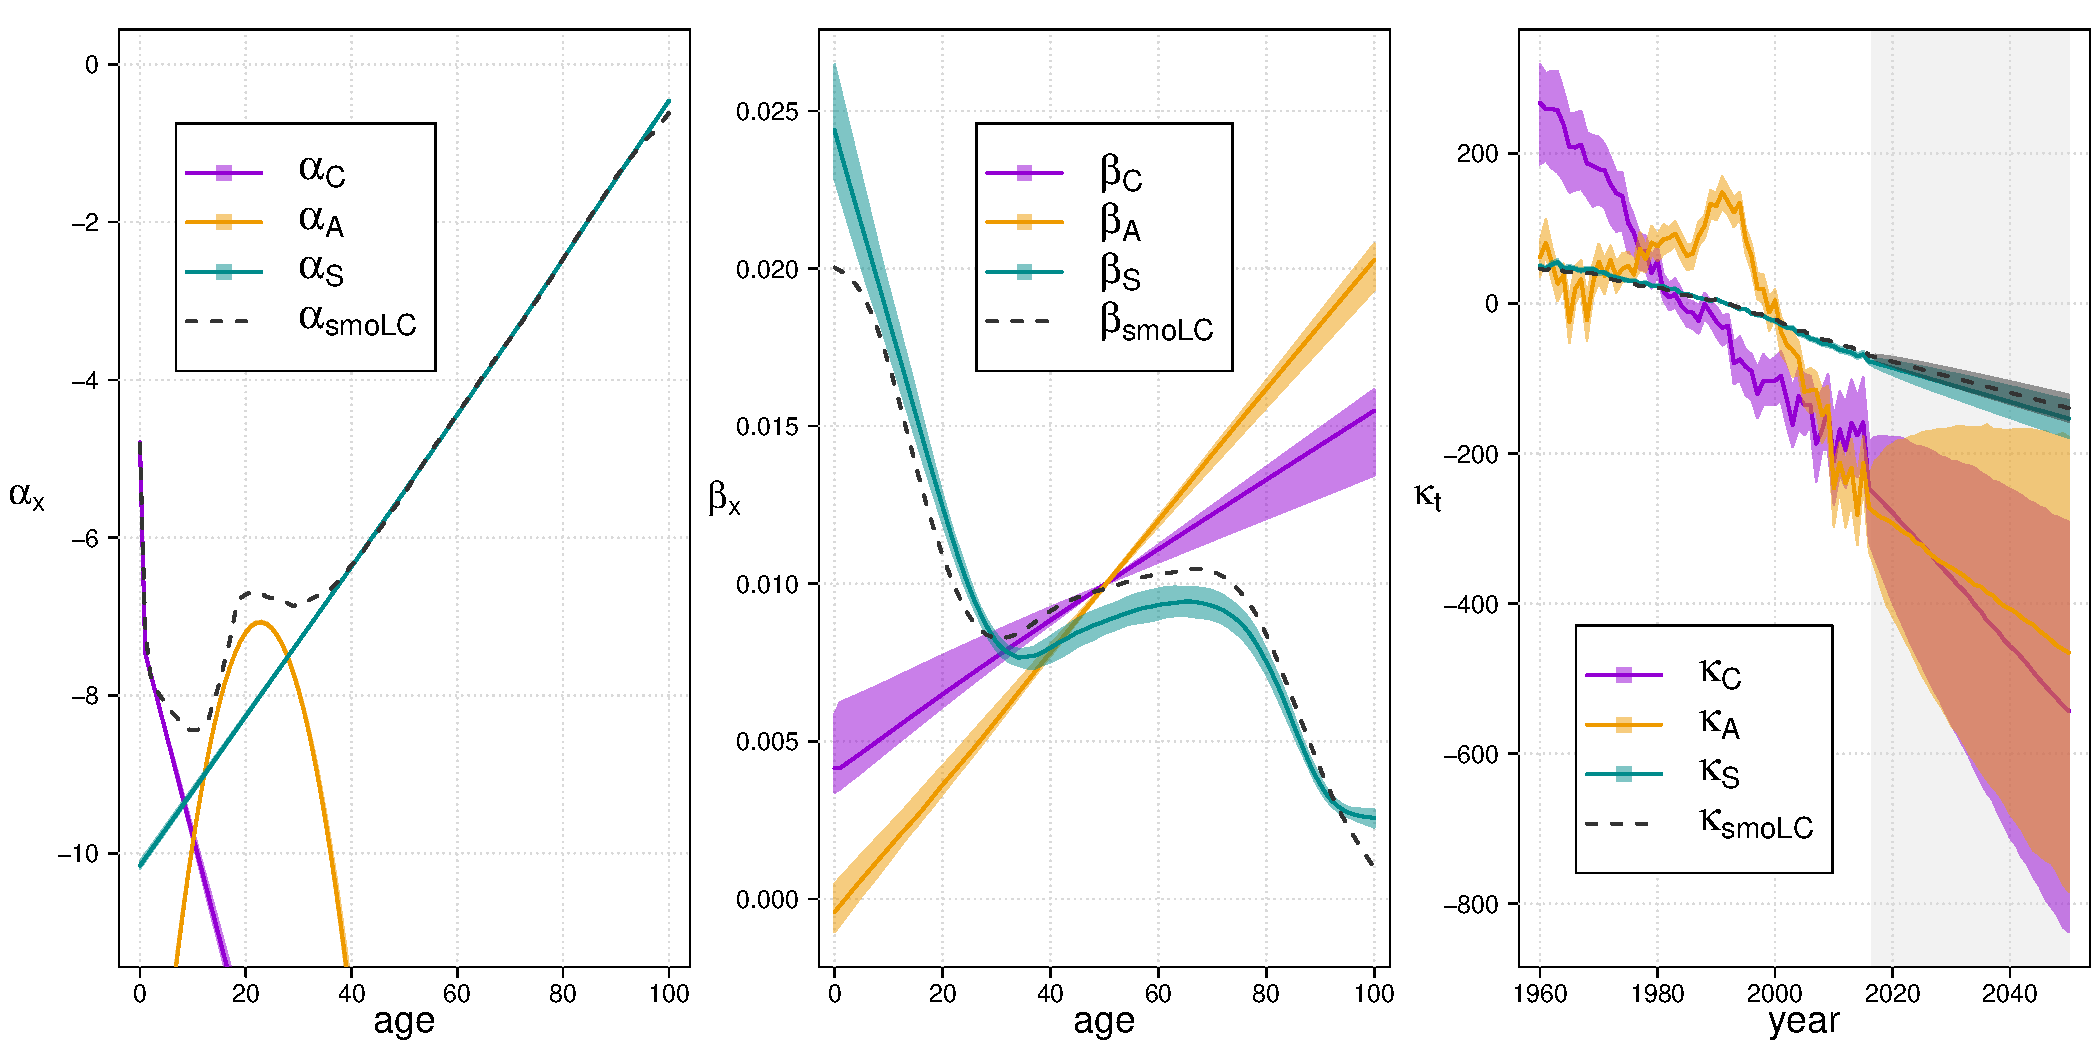
\includegraphics[scale=0.45]{./Ch6/LC3CPAR.pdf}
	\caption{\label{fig:LC3CPAR} Estimated parameters from 3C-sLC model and a smooth variant of the Lee-Carter. Swiss males, ages 0-100, years 1960-2016, time index(es) $\bm{\kappa}$ forecast up to 2050 by RWD with 80\% prediction intervals. Left panel: $\bm{\alpha}$, average shape of the age profile. Central panel: $\bm{\beta}$, age-specific average rates of mortality decline. Right panel: $\bm{\kappa}$, level of mortality at time $t$. For 3C-sLC parameters, 80\% confidence intervals are also computed for the observed years.}  
\end{figure}

Combining estimates and forecasts of the 3C-sLC parameters allows us to derive death rates for all ages and years of interest. Figure~\ref{fig:LC3COUT} shows estimated and forecast 3C-sLC death rates on a log scale for Swiss males. This figure can be directly compared with Figure~\ref{fig:LCsmoOUT}, where the respective results are shown for the smooth LC model. Several observations can be drawn from comparing the two figures. In the left panel, fitted and forecast mortality age-profiles of the 3C-sLC seem more plausible than LC ones, lacking the variable behavior and the constant age-specific rate of mortality decline of the smooth LC model. In the right panel, the superior fit of the 3C-sLC is evident, particularly at younger ages; this results from relaxing the assumption of a constant $\bm{\beta}$ in the LC framework. Age-specific mortality improvements are more flexible and produced by the combination of the component-specific parameters. The increased flexibility further translates into wider prediction intervals, which capture the uncertainty behind mortality developments at different ages.

\begin{figure}[!ht]\centering
	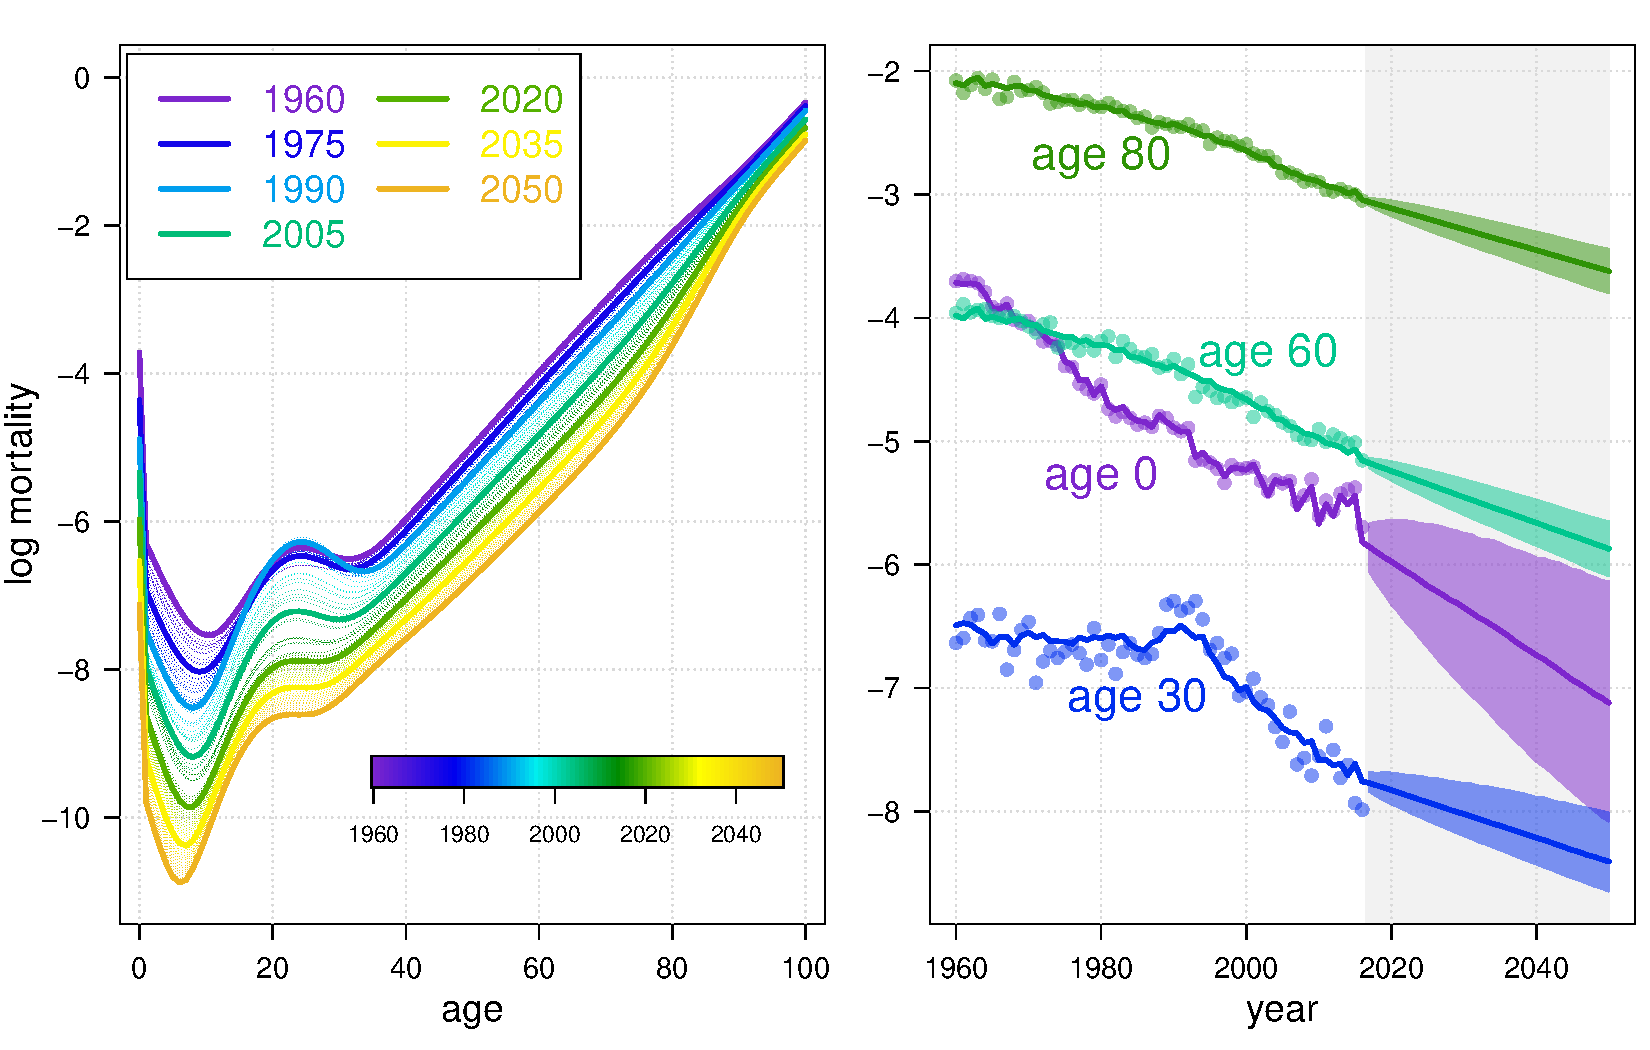
\includegraphics[scale=0.52]{./Ch6/LC3COUT.pdf}
	\caption{\label{fig:LC3COUT} Actual, estimated and forecast death rates by 3C-sLC over age and time on a log scale for Swiss males. Ages 0-100, fitted years 1960-2016, forecast years 2017-2050. Left panel: rates over age for all years. Selected years are depicted by thicker lines. Right panel: selected ages over years.}  
\end{figure}

A more rigorous assessment of the two models' goodness-of-fit is provided by comparing their deviance residuals, which are often employed as a diagnostic tool in Generalized Linear Models (GLM) settings \cite[for an overview and the formulas for their computation, please refer to][]{mccullagh1989glm}. Figure~\ref{fig:Ch6PoissonDevRes} shows the Poisson deviance residuals of the two models: the 3C-sLC displays smaller residuals than the smooth LC model, especially at childhood and early-adult ages. The red and blue clouds (corresponding to model misfit) at ages 20-40 of the smooth LC are considerably reduced in the 3C-sLC model.

\begin{figure}[!ht]\centering
	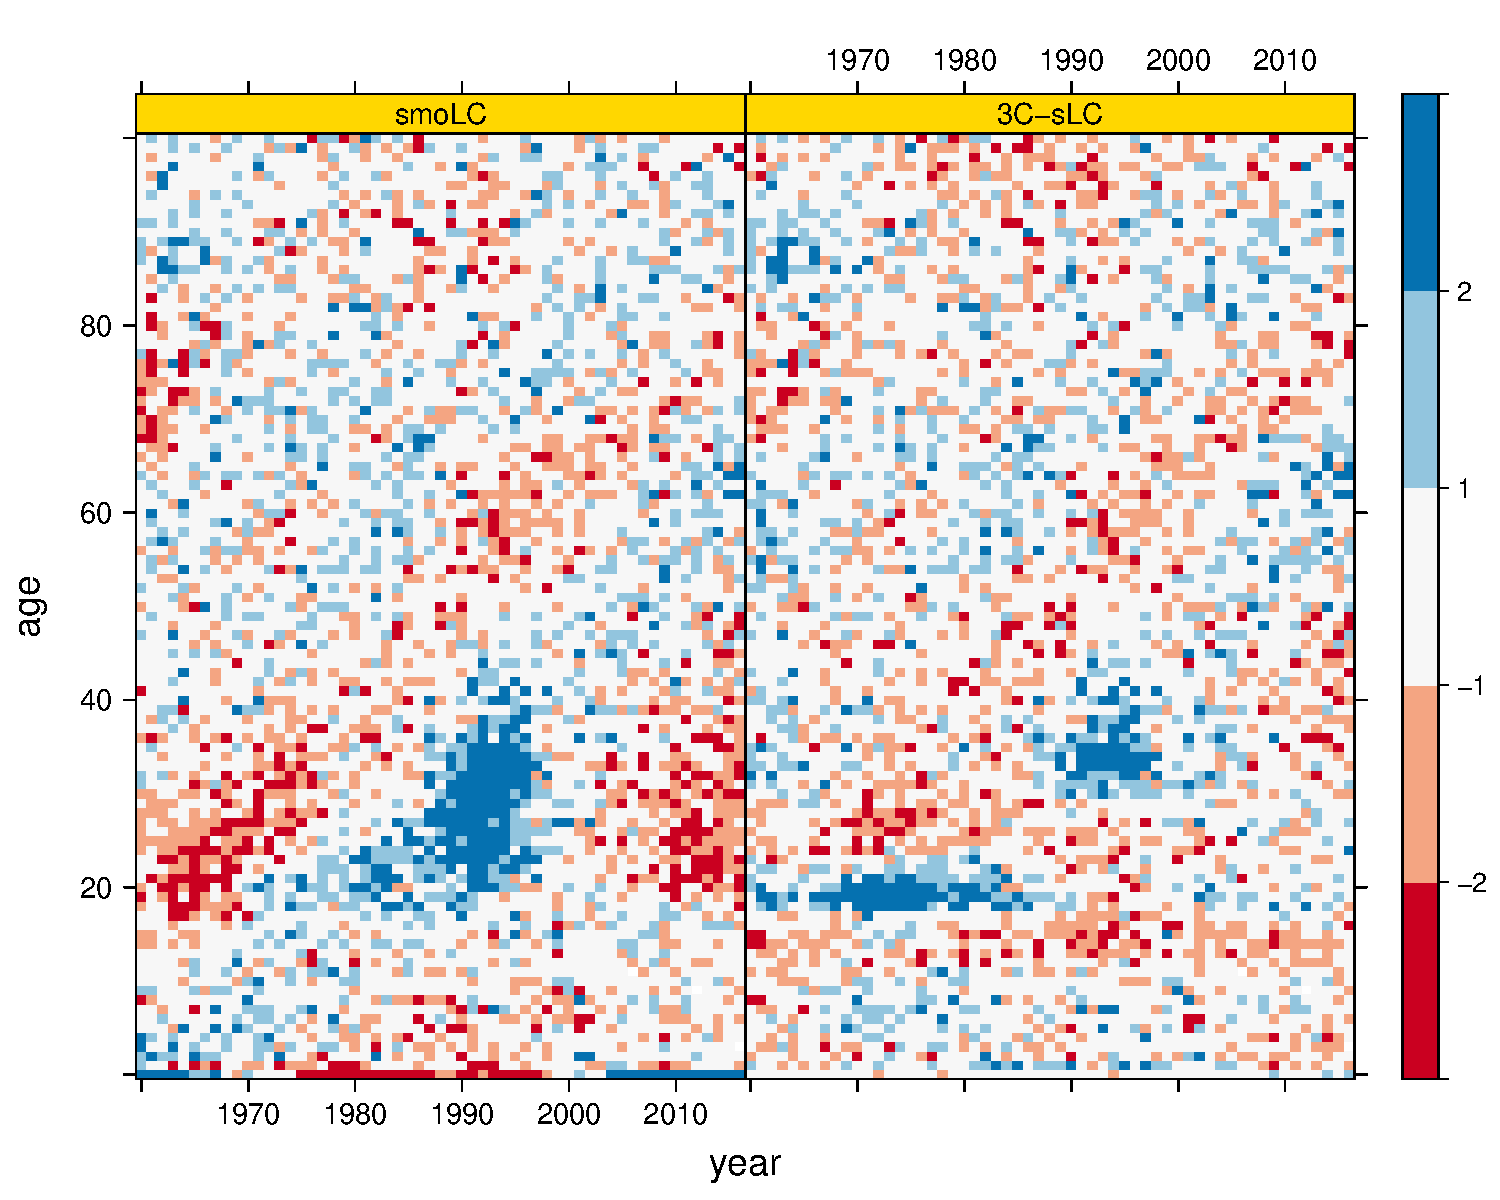
\includegraphics[scale=0.54]{./Ch6/DevResCHEm.pdf}
	\caption{\label{fig:Ch6PoissonDevRes} Poisson deviance residuals of the smooth LC and 3C-sLC models for Swiss males. Ages 0-100, fitted years 1960-2016.}  
\end{figure}

The superior fit of the 3C-sLC is a direct result of the mortality decomposition, which allows one to better describe the age-pattern of mortality. Figure~\ref{fig:3CLCcomp} displays the fitted and forecast Childhood, early-Adulthood and Senescent components on a log scale for Swiss males. The shapes observed in the $\bm{\alpha}_k$ parameters are directly carried into the mortality components. Furthermore, the central panel clearly shows the increase in early-Adulthood mortality during the years 1980-1990s, related to the strong HIV epidemic that hit this population at that time \citep{csete2012switzerland}.

\begin{figure}[!ht]\centering
	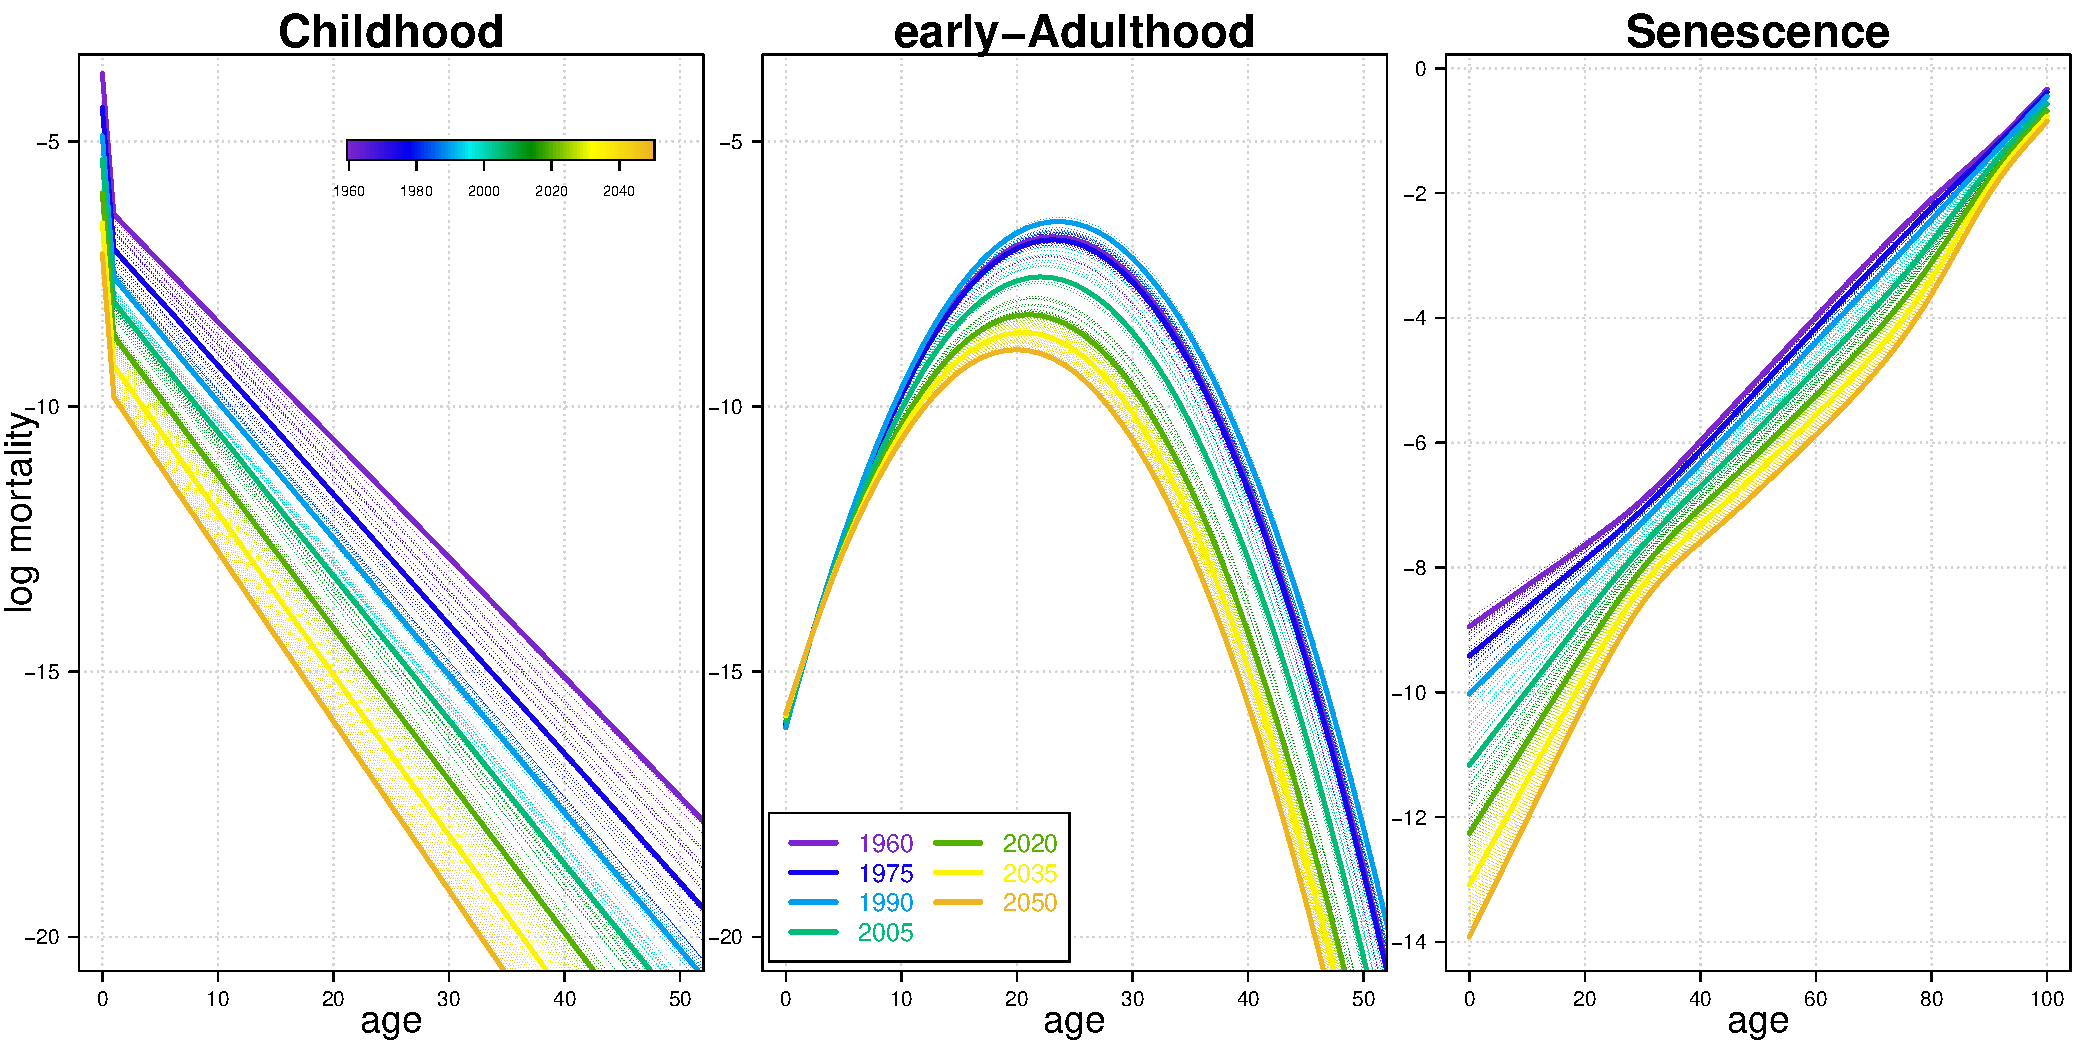
\includegraphics[scale=0.45]{./Ch6/LC3CCOMP.pdf}
	\caption{\label{fig:3CLCcomp} Estimated and forecast Childhood, Adulthood and Senescent components by 3C-sLC over age on a log scale for Swiss males. Ages 0-100, fitted years 1960-2016, forecast years 2017-2050. Axes of the left and central panels have been truncated for better displaying the mortality components.}  
\end{figure}

Next, we show the results of applying the 3C-sLC and smooth LC models to the four populations introduced in Section~\ref{Sec:Ch6sec2}, namely females and males in Switzerland (CHE) and the USA. We start by comparing the BIC values of the two models. The BIC is often used as a metric for model selection as it conveniently captures the trade-off between goodness-of-fit and parsimony of a model. Table~\ref{table:Ch6BIC} reports the BIC values for the four populations and the two models, as well as the Deviance and effective dimension (which are used to compute the BIC).  

\begin{table}[!ht]\centering
	\begin{tabular}{@{}l|rr|rr|rr@{}}
		& \multicolumn{2}{c|}{Deviance} & \multicolumn{2}{c|}{ED} & \multicolumn{2}{c}{BIC} \\ 
		& smoLC       & 3C-sLC     & smoLC      & 3C-sLC     & smoLC      & 3C-sLC     \\ \midrule
		CHE males   & 9956        & 8116       & 160        & 316        & 11340     & \textbf{10851}      \\
		\rowcolor[HTML]{EFEFEF} 
		CHE females $\;$ & 7631        & 7312       & 155       & 317        & \textbf{8975}       & 10056      \\
		USA males   & 174910      & 161476     & 221       & 311        & 176822     & \textbf{164170}     \\
		\rowcolor[HTML]{EFEFEF} 
		USA females & 91825       & 93005      & 242       & 308       & \textbf{93916}      & 95674      \\ \bottomrule
	\end{tabular}
	\caption{\label{table:Ch6BIC}Deviance, effective dimension (ED) and BIC values for the smooth LC and the 3C-sLC models for females and males in Switzerland (CHE) and the USA. Ages 0-100, fitted years 1960-2016. Lower BIC values (in bold) correspond to a  better model in terms of trade-off between accuracy and parsimony.} 
\end{table}

The table shows that the 3C-sLC is chosen over the smooth LC model by the BIC for the two male populations. Furthermore, the 3C-sLC fits the observed data better than the smooth LC model for three populations (lower values of Deviance, except for USA females), and this superior fit is a consequence of the higher number of parameters (effective dimension) employed by the 3C-sLC model.

Furthermore, we present outcomes of the 3C-sLC and smooth LC is terms of two standard and complementary summary measures of mortality. We use life expectancy at birth $e_0$ as a traditional measure of longevity and population health \citep{preston2001demogr}, and the average number of life years lost at birth $e^{\dagger}_0$ \citep{vaupel2003decomposing} as a measure of lifespan disparity. In formulas:
\begin{equation}\label{eq:e0ed}
e_0= \frac{\sum_{0}^{\omega} \ell_x}{\ell_0} \qquad \mbox{and} \qquad e^{\dagger}_0= \frac{\sum_{0}^{\omega} e_x \, d_x}{\ell_0} \, ,
\end{equation}
where $\ell_x$ denotes the life-table probability of surviving from birth to age $x$, $\ell_0$ is the life-table radix, and $\omega$ is the highest age attained in the life table. The vectors $e_x$ and $d_x$ denote the remaining life expectancy and the age-at-death distribution at age $x$, respectively. Whereas life expectancy at birth has a long tradition in measuring longevity, $e^{\dagger}_0$ has been recently employed to assess the degree of lifespan inequality within and between populations \cite[see, e.g.,][]{shkolnikov2011losses,vaupel2011life,aburto2018lifespan}, and it has also been used to evaluate mortality forecasts \citep{bohk2017lifespan,camarda2019smooth}.

Figure~\ref{fig:3CLCvsLCsmo} shows the actual $e_0$ and $e^{\dagger}_0$ for the four populations, together with the estimated and forecast values with 80\% prediction intervals for the smooth LC and 3C-sLC models. The recent flattening in $e_0$ as well as the increase in $e^{\dagger}_0$ in the USA populations, mostly caused by the increase in drug overdoses and suicides \citep{barbieri2018drug}, is evident from the figure. The wider prediction intervals of the 3C-sLC death rates (cf.~Figure~\ref{fig:LC3COUT}) translate into slightly larger intervals also for the summary mortality measures. Moreover, it is interesting to observe that forecast $e_0$ from both models are very similar, whereas forecast $e^{\dagger}_0$ differ: specifically, the 3C-sLC predicts slower mortality compression (i.e.~higher lifespan disparity) than the smooth LC. Finally, the figure shows that the models successfully capture the observed trends in $e_0$, while they are less successful for $e^{\dagger}_0$: nevertheless, the 3C-sLC performs better than the smooth LC, particularly for the Swiss populations.  

\begin{figure}[!ht]\centering
	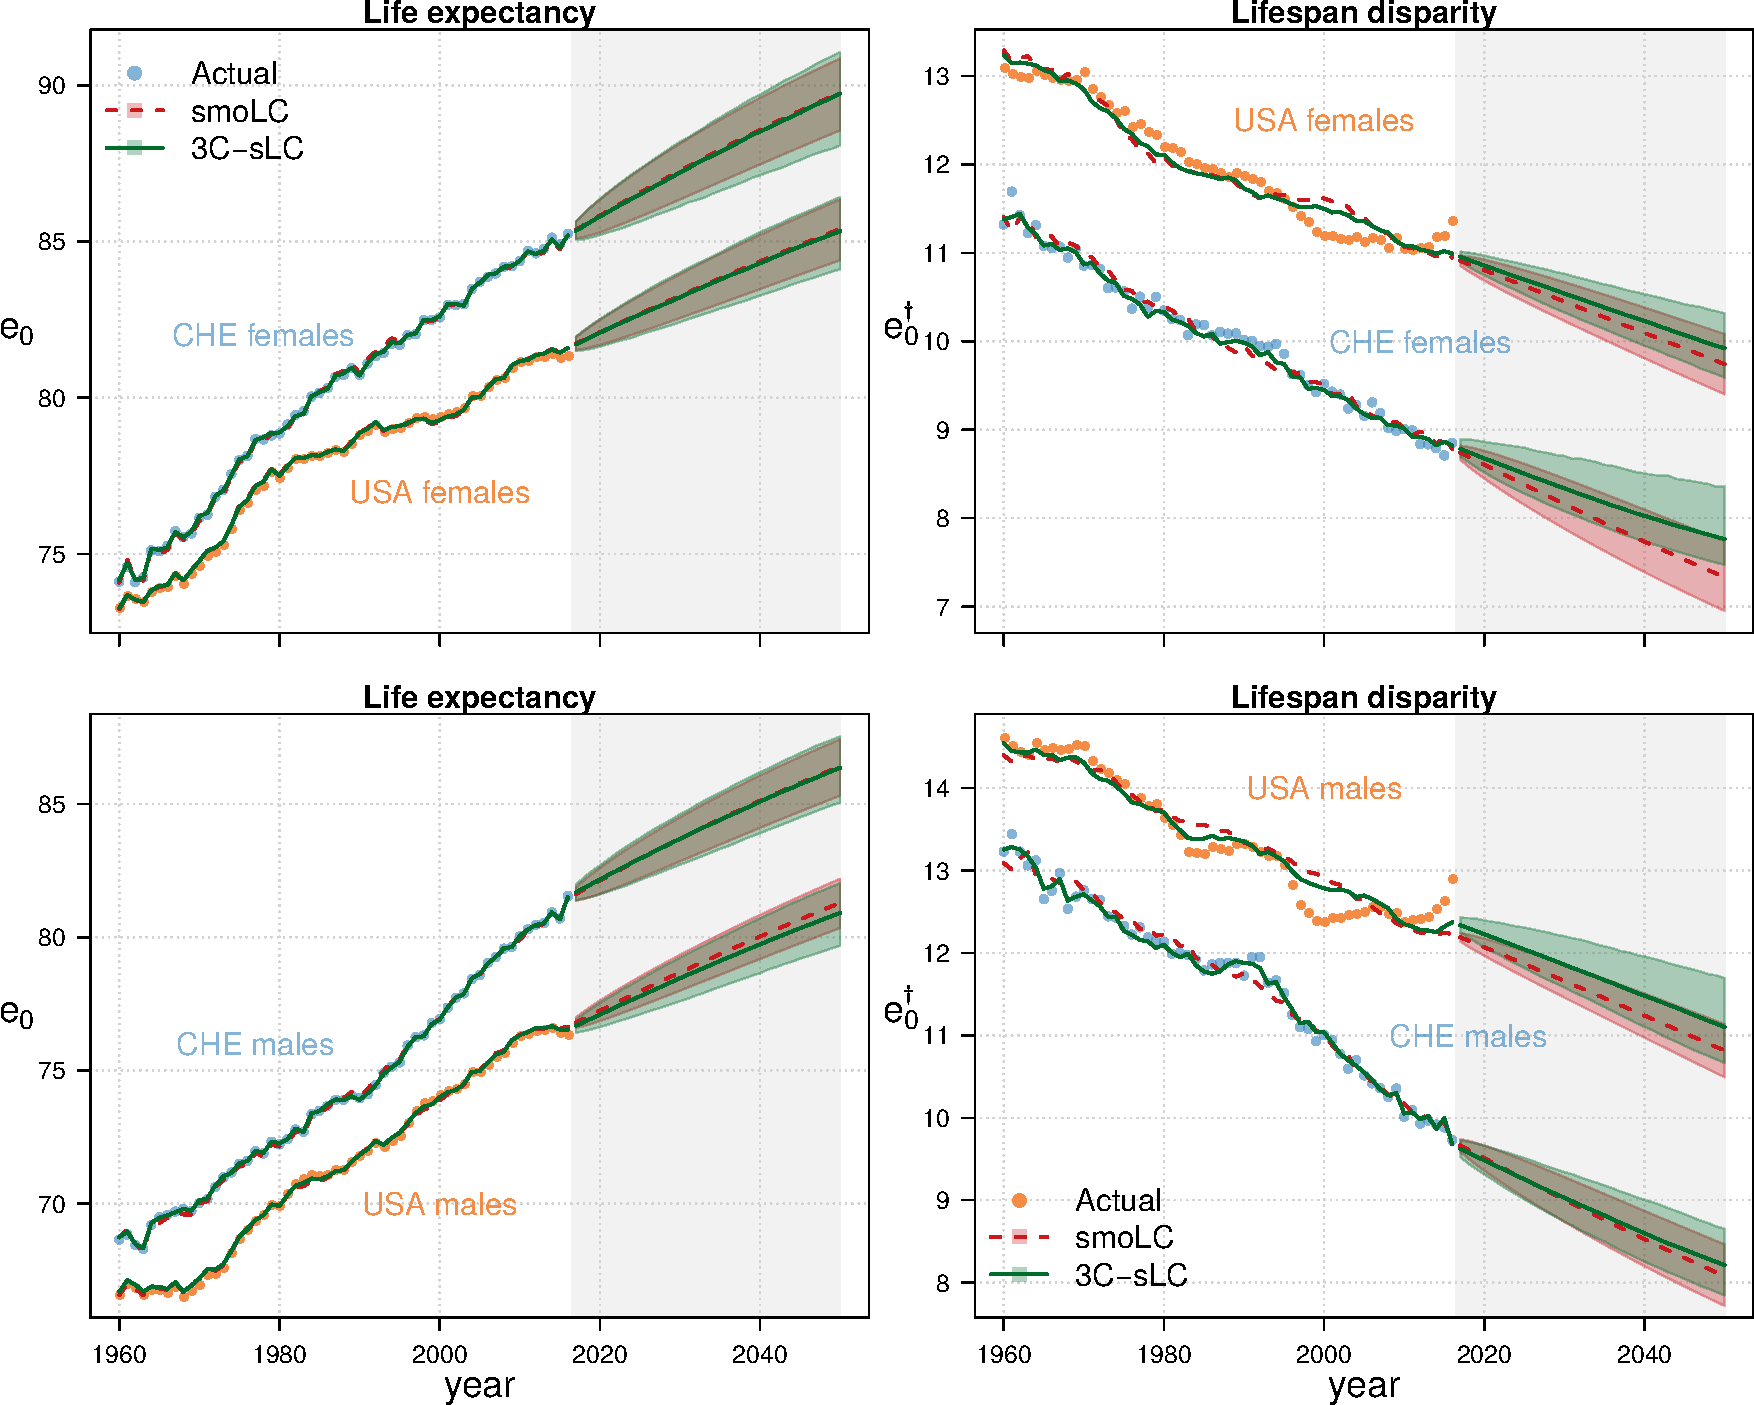
\includegraphics[scale=0.53]{./Ch6/LC3CvsSMOLC2.pdf}
	\caption{\label{fig:3CLCvsLCsmo} Actual, estimated and forecast life expectancy at birth ($e_0$, left panels) and lifespan disparity ($e^{\dagger}_0$, right panels) by smooth Lee-Carter (red lines and shades) and 3C-sLC (dark green lines and shades) with 80\% prediction intervals for females and males in Switzerland (CHE) and the USA. Ages 0-100, fitted years 1960-2016, forecast years 2017-2050.}  
\end{figure}

In order to emphasize the uniqueness of the 3C-sLC model in terms of possible outcomes, we evaluate the potential gains resulting from the hypothetical scenarios of removing one or two mortality components from the age-pattern of mortality. Specifically, we estimate the potential gains in $e_0$ and reductions in $e^{\dagger}_0$ derived from the elimination of: (i) the accident hump alone, and (ii) the accident hump together with the Childhood component. Within the 3C-sLC, these scenarios can be readily implemented by removing corresponding components (cf.~Figure~\ref{fig:3CLCcomp}) from the overall mortality pattern. Figure~\ref{fig:3CLCnoHUMP} shows the estimated and forecast 3C-sLC summary measures of mortality for males (which have a more pronounced accident hump) in Switzerland and the USA, as well as the measures computed in the two hypothetical scenarios. Removing only the accident hump would result in an average increase over the fitted periods of 0.66 and 0.63 years in $e_0$ for males in Switzerland and the USA, respectively, and in an average reduction of 0.51 and 0.47 years in $e^{\dagger}_0$. If the Childhood component were eliminated too, gains in $e_0$ would rise to 1.60 and 1.78 years in the two populations, respectively, and reductions in $e^{\dagger}_0$ would amount to 1.32 and 1.42 years. 

Moreover, the 3C-sLC allows us to decompose summary measures in future years. For instance, we forecast USA males overall life expectancy in 2050 to reach 80.92 years, with a 80\% prediction interval of $[79.68,82.03]$. The mean value of $e_0$ would increase to 81.64 if we removed only the early-Adulthood component, and to 81.89 if Childhood was excluded too. Smaller reductions are forecast for Swiss males: total life expectancy in 2050 is projected to 86.37 years $[85.05, 87.54]$, which would increase to 86.54 years if the accident hump was removed, and to 86.65 if both components were theoretically eradicated.   

\begin{figure}[!ht]\centering
	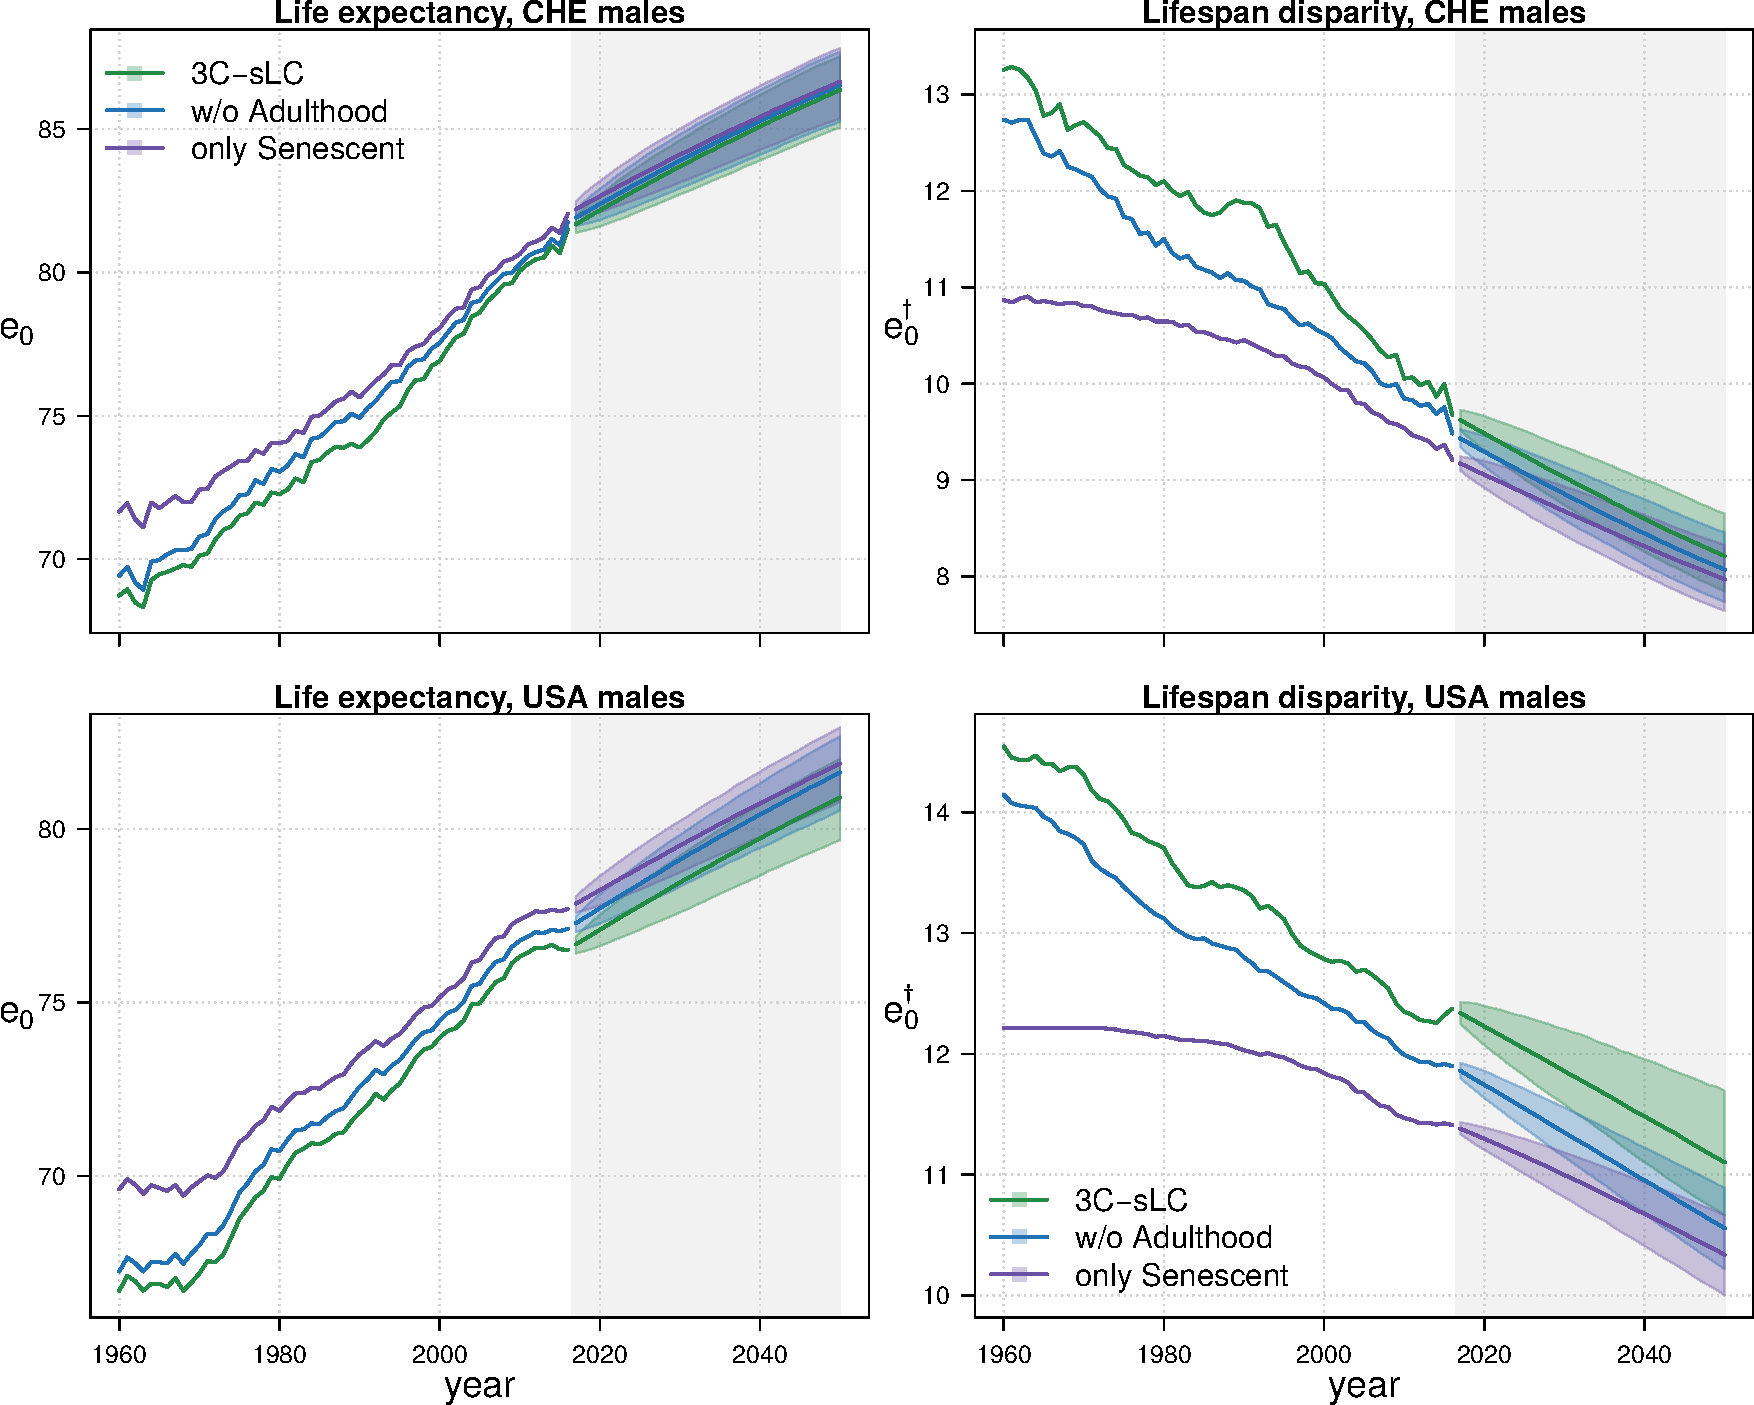
\includegraphics[scale=0.52]{./Ch6/SCENARIOS_new2.pdf}
	\caption{\label{fig:3CLCnoHUMP} Estimated and forecast life expectancy at birth ($e_0$, left panels) and lifespan disparity ($e^{\dagger}_0$, right panels) with 80\% prediction intervals by: (i) 3C-sLC (green lines and shades), (ii) 3C-sLC removing the Early-Adulthood component (blue lines and shades), and (iii) 3C-sLC removing the Childhood and Early-Adulthood components (purple lines and shades). Males in Switzerland (CHE) and the USA, ages 0-100, fitted years 1960-2016, forecast years 2017-2050.}  
\end{figure}


\section{Discussion}\label{Sec:Ch6sec4}

Models to predict the future course of mortality of rather large populations have flourished during the most recent decades, stimulated by the influential contribution of \cite{lee1992modeling}. Although the number of available approaches to forecast mortality keeps increasing by the day, the Lee-Carter (LC) model arguably remains the most widely known and adopted methodology for this purpose. At the root of this success lie two important factors, namely power and simplicity, which have made LC the benchmark approach in mortality forecasting.  

Despite its almost universal recognition and adoption, the original LC model suffers from some shortcomings (cf.~Section~\ref{Sec:Ch6sec1}). Several extensions of the model have been proposed to mitigate its principal limitations \cite[e.g.,][]{lee2001evaluating,booth2002applying,brouhns2002poisson,renshaw2006cohort,li2013extending}. However, no attempts have been made to overcome all the recognized issues simultaneously. 

In this article, we have introduced a novel generalization of the LC model that tackles all of its main limitations at once.  Starting from the hypothesis that human mortality can be conceived as the sum of three independent components \citep{thiele1871mathematical}, we propose a methodology in which mortality is simultaneously smoothed, decomposed and forecast within an LC framework. As such, we call our approach "Three-Component smooth Lee-Carter" (3C-sLC) model.

The 3C-sLC is embedded in a Poisson setting, which provides a reasonable assumption for the underlying mortality process. Smoothness in the outcomes is enforced within the estimation of the 3C-sLC parameters by employing a penalized likelihood approach. Overall mortality developments are described by the combination of three mortality components: Childhood, early-Adulthood and Senescent mortality. Each component is modelled and forecast with a smooth version of the LC model. As such, mortality developments are more flexible than in the original LC model, because they do not depend on the rather unreasonable assumption of a fixed rate of age-specific mortality improvement.   

We have shown the results of fitting and forecasting mortality with the 3C-sLC model in four populations, namely females and males in Switzerland and the USA. We have compared the 3C-sLC outcomes with those of the improved smooth version of the LC model \citep{delwarde2007smoothing}. We compared the 3C-sLC with this LC variant because both approaches are estimated in a Poisson setting with a penalized likelihood for enforcing smooth outcomes. Moreover, it should be noted that this comparison could have been made only at the overall mortality level: all LC variants as well as other existing forecasting models do not allow one to simultaneously forecast and decompose mortality into meaningful components. For the same reasons, additional comparisons and out-of-sample exercises would have assessed performances of the 3C-sLC only for one of its features, underrating its great explanatory value.

At the overall mortality level, the 3C-sLC death rates fit observed mortality developments better than the smooth LC model; moreover, 3C-sLC forecast rates are characterized by wider prediction intervals, which result from the enhanced flexibility of the model. This is a potential advantage of the 3C-sLC model, as LC prediction intervals have been criticized for being too narrow \citep{alho1992comment}. Although the 3C-sLC generally fits better the observed mortality data, the smooth LC model was preferred by the BIC criterion for the female populations. A potential explanation for this is that the accident hump is not a relevant feature of the mortality pattern for females analysed in this article. We plan to investigate modelling and forecasting female mortality using only two  components (i.e.~Childhood and Senescence) in future work.

For both models, we have further computed and compared two complementary summary measures of mortality: life expectancy at birth ($e_0$) and lifespan disparity at birth ($e^{\dagger}_0$). The two measures provide information on the longevity and lifespan inequality  of the population. Despite being characterized by rather similar fitted and forecast values of $e_0$, the difference between the two models clearly emerges from $e^{\dagger}_0$. The 3C-sLC better captures observed trends in lifespan inequality, and it forecasts slower mortality compression than the smooth LC model. This is another advantage of the 3C-sLC, since LC forecasts have been shown to produce a (possibly) too fast mortality compression \cite[see, e.g.,][]{bardoutsos2018projecting,basellini2019modelling}. In terms of prediction intervals, the widening observed in 3C-sLC rates only partially carries forward to forecast $e_0$ and $e^{\dagger}_0$; the reason is that larger 3C-sLC intervals occur at younger ages especially, whose influence on summary mortality measures is rather limited. 

Comparing the two models' estimated parameters (cf.~Figure~\ref{fig:LC3CPAR}) provides two interesting points for discussion. First, the 3C-sLC estimates of the Senescent component closely mirror those of the smooth LC model (with the exception of the $\bm{\hat{\alpha}}$ values at young and early-adult ages). This hints at the fact that the LC model is driven by the Senescent component of mortality, which carries most weight in terms of death counts. Within the standard (or improved) LC framework, mortality developments of Childhood and early-Adulthood components are thus conflated with Senescent ones, resulting in a loss of fitting accuracy. The second point worthy of discussion concerns the variability of the 3C-sLC model. Figure~\ref{fig:LC3CPAR} shows that confidence intervals for the $\bm{\alpha}_k$ estimates are very narrow. Hence, uncertainty in the 3C-sLC model depends on the variability of the $\bm{\beta}_k$ and $\bm{\kappa}_k$ estimates.

The presence of three independent components could prompt a reader to establish an association between the 3C-sLC and LC variants with additional $\beta^{(i)}_x \kappa^{(i)}_t$ interaction terms \citep{renshaw2003lee, hyndman2007robust}. However, the two approaches present substantial differences in both methodological and demographic perspectives. Whereas the 3C-sLC attempts to decompose the mortality pattern into additive independent components, the LC model (with more interaction terms) tries to approximate it with additional terms that have decreasing explicative power. In statistical terms, the 3C-sLC models the expected values of the Poisson process, while the LC models the logarithm of the expected values \cite[for a more detailed discussion in a general modelling framework, see][p.~279]{camarda2016sums}.

The decomposition of mortality into its three independent components has received considerable interest during recent decades (cf.~Section~\ref{Sec:Ch6sec1}). However, only a few methodologies have been proposed to take into account the three components when projecting mortality. The well-established model of  \cite{heligman1980age} has only been employed by \cite{forfar1987changing} in mortality projections due to the high number of parameters to forecast. Moreover, \cite{bardoutsos2018projecting} employed the ten-parameter CoDe model \citep{de2016new} to forecast the full age range of mortality. The authors find that accounting for the compression and delay (i.e.~shift) of mortality improves point forecast accuracy with respect to the LC model when the modal age at death increases linearly. Finally, \cite{basellini2019three} proposed the 3C-STAD model to analyze and forecast component-specific age-at-death distributions derived from a non-parametric decomposition of the mortality pattern. The authors show that 3C-STAD projections for high-longevity populations are more accurate in terms of point forecasts and prediction intervals than the LC model and its variants. 

The mortality decomposition provides interesting demographic insights into fitted and forecast mortality schedules. The increased quantity of information on component-specific patterns allows one to obtain a more thorough overview on mortality developments. Furthermore, hypothetical exercises can readily be performed within this framework. For example, it is possible to estimate the potential gains in $e_0$ and reductions in $e^{\dagger}_0$ resulting from the elimination of one or more mortality components. We have performed this exercise for the male populations analysed in this article: for the observed period, we estimate an average 1.60 and 1.78 additional years of longevity in Switzerland and the USA, respectively, and an average 1.32 and 1.42 reduced years of lifespan disparity by theoretically eradicating the Childhood and early-Adulthood components. We present similar analysis for the forecast years too.

Two additional findings related to these exercises deserve mention. Firstly, Figure~\ref{fig:3CLCnoHUMP} shows that the Childhood and early-Adulthood components have a significant effect on $e_0$ and $e^{\dagger}_0$ for both male populations during the fitted years only. In forecast years, the effect of the two components varies by population: in Switzerland, the two forecast scenarios converge to the baseline mortality pattern, while in the USA differences between the scenarios do not disappear. Forecast Childhood and early-Adulthood components thus seem to maintain a significant role only in the USA. Secondly, the bottom panels of Figure~\ref{fig:3CLCnoHUMP} highlight that lifespan disparity fluctuations are driven by the Childhood and early-Adulthood components: removing them from the age-pattern of mortality smooths the trends of  $e^{\dagger}_0$ in both populations. 


\section{Conclusions}\label{Sec:Ch6sec5}

The proposed 3C-sLC aims to provide demographers and actuaries with a new extension of the LC model that overcomes its main drawbacks while maintaining the factors that underpin its success. Conceptually, the 3C-sLC can be thought of as the combination of three LC models, each one targeted to model and forecast the Childhood, early-Adulthood and Senescent components of mortality. We thus keep the simplicity of the LC framework, namely the interpretability of the three set of parameters $\alpha_x$, $\beta_{x}$ and $\kappa_{t}$ (one triplet for each mortality component). Furthermore, forecasting is performed as in the original LC model, without introducing additional layers of complexity. Although the formulas developed to fit the 3C-sLC are somewhat more elaborate than the original SVD decomposition suggested by \cite{lee1992modeling}, we provide the routines needed to fit and forecast mortality with our proposed model in the Supplementary Material to this article. Our hope is that the 3C-sLC could be employed by researchers and statistical agencies that currently use the LC model in an effort to obtain more desirable outcomes within the same LC framework.

\cleardoublepage

\end{document}